%%
%% This is file `sample-sigconf.tex',
%% generated with the docstrip utility.
%%
%% The original source files were:
%%
%% samples.dtx  (with options: `sigconf')
%% 
%% IMPORTANT NOTICE:
%% 
%% For the copyright see the source file.
%% 
%% Any modified versions of this file must be renamed
%% with new filenames distinct from sample-sigconf.tex.
%% 
%% For distribution of the original source see the terms
%% for copying and modification in the file samples.dtx.
%% 
%% This generated file may be distributed as long as the
%% original source files, as listed above, are part of the
%% same distribution. (The sources need not necessarily be
%% in the same archive or directory.)
%%
%% The first command in your LaTeX source must be the \documentclass command.
\documentclass[10pt,sigconf,letterpaper]{acmart}
\acmYear{2019}
\copyrightyear{2019}
\acmConference{CoNEXT '19}{December 9-12, 2019}{Orlando, Florida, USA}

\usepackage{multirow}
\usepackage{blindtext}

%\settopmatter{printacmref=false} % Removes citation information below abstract
%\renewcommand\footnotetextcopyrightpermission[1]{} % removes footnote with conference information in first column

\newcommand\note[2]{{\color{#1}#2}}
\newcommand\todo[1]{{\note{red}{TODO: #1}}}

%%
%% \BibTeX command to typeset BibTeX logo in the docs
\AtBeginDocument{%
  \providecommand\BibTeX{{%
    \normalfont B\kern-0.5em{\scshape i\kern-0.25em b}\kern-0.8em\TeX}}}


%%
%% Submission ID.
%% Use this when submitting an article to a sponsored event. You'll
%% receive a unique submission ID from the organizers
%% of the event, and this ID should be used as the parameter to this command.
%%\acmSubmissionID{123-A56-BU3}

%%
%% The majority of ACM publications use numbered citations and
%% references.  The command \citestyle{authoryear} switches to the
%% "author year" style.
%%
%% If you are preparing content for an event
%% sponsored by ACM SIGGRAPH, you must use the "author year" style of
%% citations and references.
%% Uncommenting
%% the next command will enable that style.
%%\citestyle{acmauthoryear}

%%
%% end of the preamble, start of the body of the document source.
\begin{document}

%%
%% The "title" command has an optional parameter,
%% allowing the author to define a "short title" to be used in page headers.
\title{Bricking up and overgrowing backdoors in Intrusion Detection Systems}

\begin{abstract}
Interest in poisoning attacks and backdoors recently resurfaced for Deep Learning (DL) applications. Several successful defense mechanisms have been recently proposed for Convolutional Neural Networks, for example in the context of autonomous driving. We show that, surprisingly, common defense mechanisms fail utterly to remove backdoors in DL for Intrusion Detection Systems. However, we find that visualization approaches can aid in identifying a backdoor independent of the used classifier. Finally, we conceive pruning-based approaches to remove backdoors for decision trees and random forests and demonstrate their effectiveness for several network security datasets. 
\end{abstract}

%%
%% The "author" command and its associated commands are used to define
%% the authors and their affiliations.
%% Of note is the shared affiliation of the first two authors, and the
%% "authornote" and "authornotemark" commands
%% used to denote shared contribution to the research.
\author{Maximilian Bachl}
\affiliation{\institution{Technische Universit\"at Wien}}
%\authornote{Both authors contributed equally to this research.}
\email{maximilian.bachl@tuwien.ac.at}

\author{Alexander Hartl}
\affiliation{\institution{Technische Universit\"at Wien}}
%\authornotemark[1]
\email{alexander.hartl@tuwien.ac.at}

\author{Tanja Zseby}
\affiliation{\institution{Technische Universit\"at Wien}}
\email{tanja.zseby@tuwien.ac.at}

\author{Joachim Fabini}
\affiliation{\institution{Technische Universit\"at Wien}}
\email{joachim.fabini@tuwien.ac.at}

%%
%% By default, the full list of authors will be used in the page
%% headers. Often, this list is too long, and will overlap
%% other information printed in the page headers. This command allows
%% the author to define a more concise list
%% of authors' names for this purpose.
%\renewcommand{\shortauthors}{Hartl and Bachl}

%%
%% The abstract is a short summary of the work to be presented in the
%% article.
%\begin{abstract}
%  A clear and well-documented \LaTeX\ document is presented as an
%  article formatted for publication by ACM in a conference proceedings
%  or journal publication. Based on the ``acmart'' document class, this
%  article presents and explains many of the common variations, as well
%  as many of the formatting elements an author may use in the
%  preparation of the documentation of their work.
%\end{abstract}

\settopmatter{printfolios=true}
\maketitle

\todo{We should only add the backdoor in forward direction actually. But it doesn't really matter I guess.}

\section{Introduction}
The detection of attacks in data networks is a fundamental task in data security. Due to the considerable amount of data which has to be analyzed the use of machine learning techniques for this purpose seems natural and is increasingly deployed.

For research, the invention and assessment of techniques for network anomaly detection poses many challenges. To implement such a system, a considerable number of features can be extracted from network data which might be beneficial for anomaly detection and it is not always clear which features are actually important. 

For the training of models usually datasets are used which have been generated artificially in a controlled test environment. As a downside of this approach, it is unclear whether a machine learning model learns to classify based on characteristics that are inherent to the attacks which should be detected, or rather learns to classify based on patterns that were unintentionally created during dataset generation.

For a well-performing network anomaly detection technique it is therefore of utmost importance to study which patterns the technique looks at to distinguish attack traffic from normal traffic, and question if these explanations match with expert knowledge.

% TODO: think Fares didnt use this
In this document, we redo parts of a recent paper~\cite{fares} which bases on the CIC-IDS-2017 dataset \cite{Sharafaldin2018} for evaluating the performance of several feature vectors and machine learning techniques for accurate anomaly detection. We use explainability methods for investigating if the decisions the anomaly detectors untertake are reasonable.

Furthermore, we add a backdoor to the trained model and show that attack detection can efficiently be bypassed if the attacker had the ability to modify training data. Finally, we apply the same explainability methods to the backdoored model and show how such attack attempts might be recognized before any harm is done.


\begin{table}[b]
\caption{Detection performance results.} \label{tab:performance_results}
\begin{tabular}{l r r} \toprule
& Random Forest & Deep Learning \\ \midrule
Accuracy	&	0.9974 $\pm$ 0.0001	&	0.9970 $\pm$ 0.0002	\\
Precision	&	0.9965 $\pm$ 0.0001	&	0.9979 $\pm$ 0.0001	\\
Recall	&	0.9931 $\pm$ 0.0002	&	0.9903 $\pm$ 0.0007	\\
F1	&	0.9948 $\pm$ 0.0001	&	0.9941 $\pm$ 0.0004	\\
Youden	&	0.9920 $\pm$ 0.0002	&	0.9896 $\pm$ 0.0007	\\
\bottomrule
\end{tabular}
\end{table}

\section{Related Work}

\section{Anomaly Detection Approaches} \label{sec:ml_approaches}
\subsection{Datasets}
Several datasets for the purpose of building and evaluating IDSs have been developed. However, as pointed out in \cite{gharib2016}, there are numerous requirements that have to be met for a dataset to provide realistic performance benchmarks in this context.

In this research, we use the UNSW-NB15~\cite{moustafa2015unsw} and the CIC-IDS-2017~\cite{Sharafaldin2018} datasets, which were developed by two independent institutions and are both freely available on the Internet, guaranteeing reproducibility of our results.

The UNSW-NB15 dataset~\cite{moustafa2015unsw} was created by researchers of the University of New South Wales to overcome common problems due to outdated datasets. Network captures containing over 2 million flows of normal traffic and various types of attacks are provided together with a ground truth file. Attack traffic includes exploits, fuzzers, reconnaissance attacks, DoS attacks, shellcode, analysis attacks, backdoors and worms.

The CIC-IDS-2017 dataset~\cite{Sharafaldin2018} was created by the Canadian Institute of Cybersecurity to provide an alternative to existing datasets which are found to exhibit several shortcomings. The provided raw network captures contain over 2.3 million flows, containing both normal traffic and attacks, which can be coarsely classified into DoS attacks, infiltration attacks, web attacks, brute force and scanning attacks.

We base our analysis on the CAIA~\cite{Williams2006} feature vector as formulated in~\cite{fares}, which thus includes the used protocol, flow duration, packet count and the total number of transmitted bytes, the minimum, maximum, mean and standard deviation of packet length and inter-arrival time and the number of packets with specific TCP flags set. All features except protocol and flow duration are evaluated for forward and backward direction separately. The goal of this research is to investigate the possibility of poisoning attacks. We therefore also include the minimum, maximum and standard deviation of TTL values in our feature vector as an attractive carrier for exploitation as a backdoor. % TODO: justify use of TTL better

We used the go-flows~\cite{goflows} flow exporter for extracting these features from the raw capture files, applied Z-score normalization to process the data and used 3-fold cross validation for evaluating the models' performances.

% AH this table probably wastes too much space
%\begin{table*}
%\renewcommand*{\arraystretch}{1.2} % TODO: better order
%\caption{Flow features used for attack detection.}
%\label{tab:features}
%\begin{tabular}{l l l l l} \toprule
%dstBytes	&	max\_srcPktLength	&	min\_dstPktIAT	&	srcPkts	&	\#dstTCPflag:ack	\\
%dstPkts	&	max\_srcTTL	&	min\_dstPktLength	&	srcPort	&	\#dstTCPflag:cwr	\\
%dstPort	&	mean\_dstPktIAT	&	min\_dstTTL	&	stdev\_dstPktIAT	&	\#dstTCPflag:fin	\\
%duration	&	mean\_dstPktLength	&	min\_srcPktIAT	&	stdev\_dstPktLength	&	\#dstTCPflag:syn	\\
%max\_dstPktIAT	&	mean\_dstTTL	&	min\_srcPktLength	&	stdev\_dstTTL	&	\#srcTCPflag:ack	\\
%max\_dstPktLength	&	mean\_srcPktIAT	&	min\_srcTTL	&	stdev\_srcPktIAT	&	\#srcTCPflag:cwr	\\
%max\_dstTTL	&	mean\_srcPktLength	&	protocol	&	stdev\_srcPktLength	&	\#srcTCPflag:fin	\\
%max\_srcPktIAT	&	mean\_srcTTL	&	srcBytes	&	stdev\_srcTTL	&	\#srcTCPflag:syn	\\
% \bottomrule
%\end{tabular}
%\end{table*}
 
\subsection{Deep Learning}
We used PyTorch to build a neural network classifier. For this we used 5 fully connected layers with 512 neurons each and applied ReLU after each layer as well as dropout with a probability of 0.2. We use the binary cross entropy loss function for the classification task itself. 

\subsection{Random Forests}
In addition to deep learning we trained a random forest classifier to detect attacks in network traffic. We used the RandomForestClassifier implementation from scikit-learn for this task and used 100 estimators for training each random forest.


\subsection{Performance Results}
Table~\ref{tab:performance_results} shows performance results for both deep learning and random forests. Our results are consistent with previous work like, e.g., \cite{fares}.



\section{Explainability Plots} \label{sec:plots}
Several graphs have been proposed for visualizing feature dependence of non-interpretable machine learning models~\cite{goldstein2015peeking, friedman2001greedy, apley2016visualizing}.
In this section, we introduce the graphs which we will use for interpreting our models' outcomes which are not available in real-world situations.
\subsection{Partial Dependence Plots}
Partial Dependence Plots (PDP) were proposed in \cite{friedman2001greedy} and visualize dependence of a model's predictions by plotting the model's prediction for a modified dataset for which the feature's value has been fixed to a certain value and computing the an average over the dataset.

If we denote by $\boldsymbol X \in \mathbb R ^n$ a random vector drawn from the feature space and by $f(\boldsymbol X) \in [0,1]$ the  prediction function, the PDP for the $i$th feature $X_i$ can be expressed as
\begin{equation}
\text{PDP}_i(y) = \mathbb E_{\boldsymbol X}\left(f(X_1,\ldots,X_{i-1},y,X_{i+1},\ldots X_n)\right) . % \int _{\mathbb R^n} Predict(x_1,\ldots,x_{i-1},y,x_{i+1},\ldots x_n) f(\boldsymbol x) d\boldsymbol x .
\end{equation}
Empirically, we can approximate the distribution of the feature space using the distribution of observed samples. Hence, at a given point $y,$ the PDP can be found by setting the corresponding value of all samples in the dataset to $y$ and averaging over the predictions of the resulting modified dataset.

\subsection{Individual Conditional Expectation}
The averaging which is done for PD plots introduces the problem that the influence of a feature on individual samples is lost. In our case, the predictions of both deep learning and random forests turned out to be strongly dependent on other features as well \todo{How do we see that?}. Hence, by averaging information gets lost and wrong explanations might be the consequence.

For this reason, Individual Conditional Expectation (ICE) plots were proposed \cite{goldstein2015peeking}. For ICE plots, we omit averaging over multiple samples and plot the effect of modifying one feature value for  individual samples directly, i.e. for a particular sample $\boldsymbol x$ we can compute an ICE plot as

\begin{equation}
\text{ICE}_i(y, \boldsymbol x) = f(x_1,\ldots,x_{i-1},y,x_{i+1},\ldots x_n).
\end{equation}

\subsection{Accumulated Local Effects}
Due to feature dependence it is very likely that in the feature space areas exist which have a very low probability to occur. Since a model is trained with real, observed data, the training set therefore does not include samples for these areas, which causes the model's predictions to become indeterminate for these areas. This poses a problem when considering these predictions for computing PDPs. 

In an attempt to overcome this problem, it is possible to only consider samples which are likely to occur for certain feature values, i.e. to consider the conditional distribution of remaining features, for computing explainability graphs. This results the concept for Accumulated Local Effects (ALE) plots. 

For the $i$th feature $X_i$, the ALE plot ALE$_i(y)$ can be defined differentially as



\begin{equation}
\frac{d}{dy} \text{ALE}_i (y) = \mathbb E_{\boldsymbol X | X_i}\left(\frac{d}{dy} f(X_1,\ldots,X_{i-1},y,X_{i+1},\ldots X_n) | X_i=y\right)
\end{equation}
\todo{I think that there are some minor problems with $y$ and $X_i$ in the formula.}

To combat ambiguity of this definition, we force ALE$_i(x)$ to have zero mean on the domain of $X_i$.

For empirical evaluation, we approximate the conditional distributions of $\boldsymbol X$ by averaging over samples for which $X_i \approx y$. 

When computing ALE plots, we experienced the problem of empty intervals. If there are intervals  that do not contain any values, the usual definition which takes values between the interval's boundaries for estimating the conditional probability density for feature values doesn't work. 

For this reason, we modified this definition to instead use the closest 10 samples to the interval's center for estimating the distribution.

\subsection{Interpretation}
\subsubsection{PDPs}

\begin{figure*}[p]
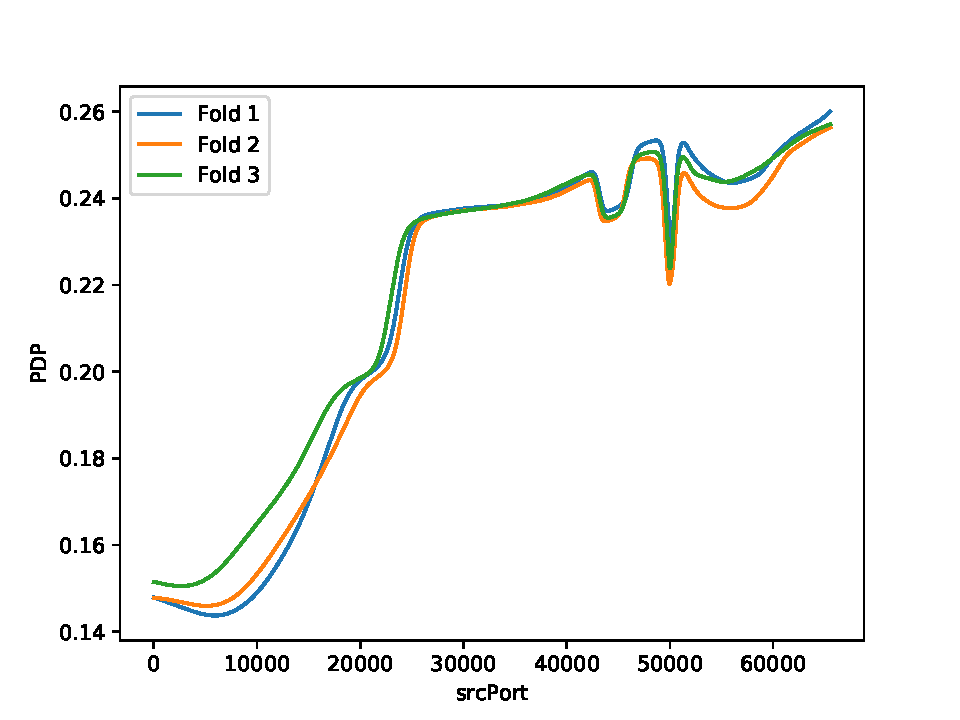
\includegraphics[width=0.48\textwidth]{../pdp_CAIA_backdoor_17/sourceTransportPort_nn.pdf}
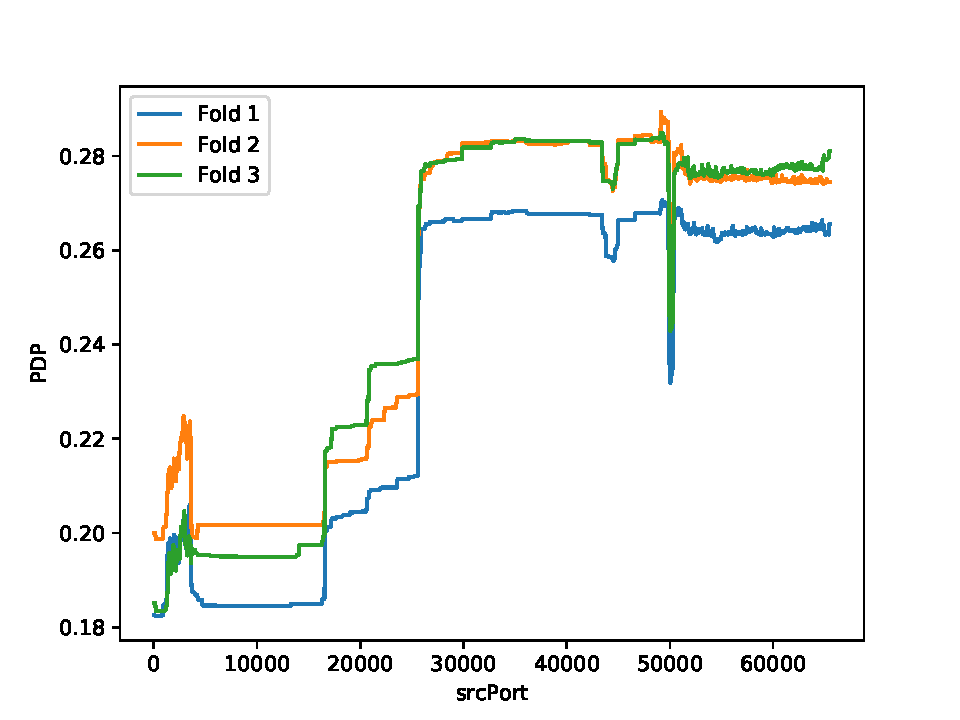
\includegraphics[width=0.48\textwidth]{../pdp_CAIA_backdoor_17/sourceTransportPort_rf.pdf}

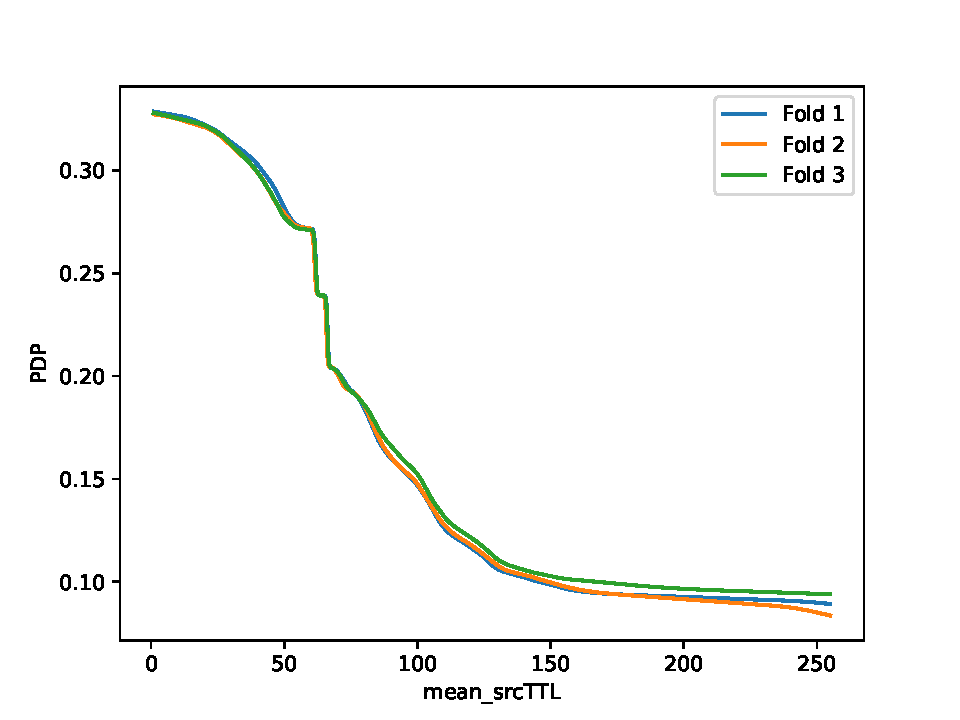
\includegraphics[width=0.48\textwidth]{../pdp_CAIA_backdoor_17/apply(mean(ipTTL),forward)_nn.pdf}
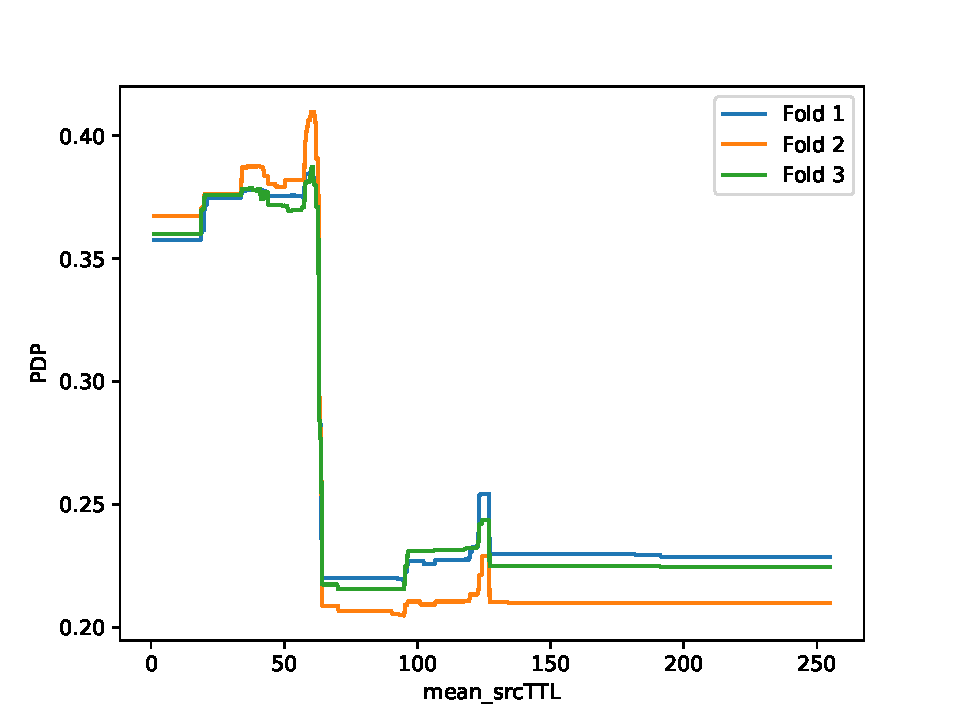
\includegraphics[width=0.48\textwidth]{../pdp_CAIA_backdoor_17/apply(mean(ipTTL),forward)_rf.pdf}

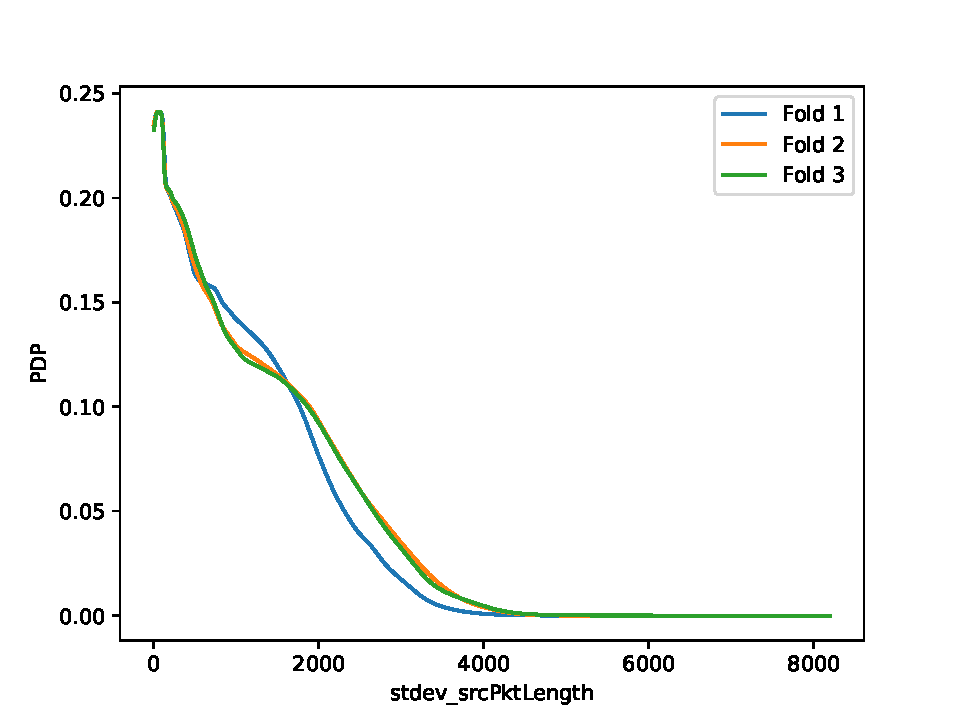
\includegraphics[width=0.48\textwidth]{../pdp_CAIA_backdoor_17/apply(stdev(ipTotalLength),forward)_nn.pdf}
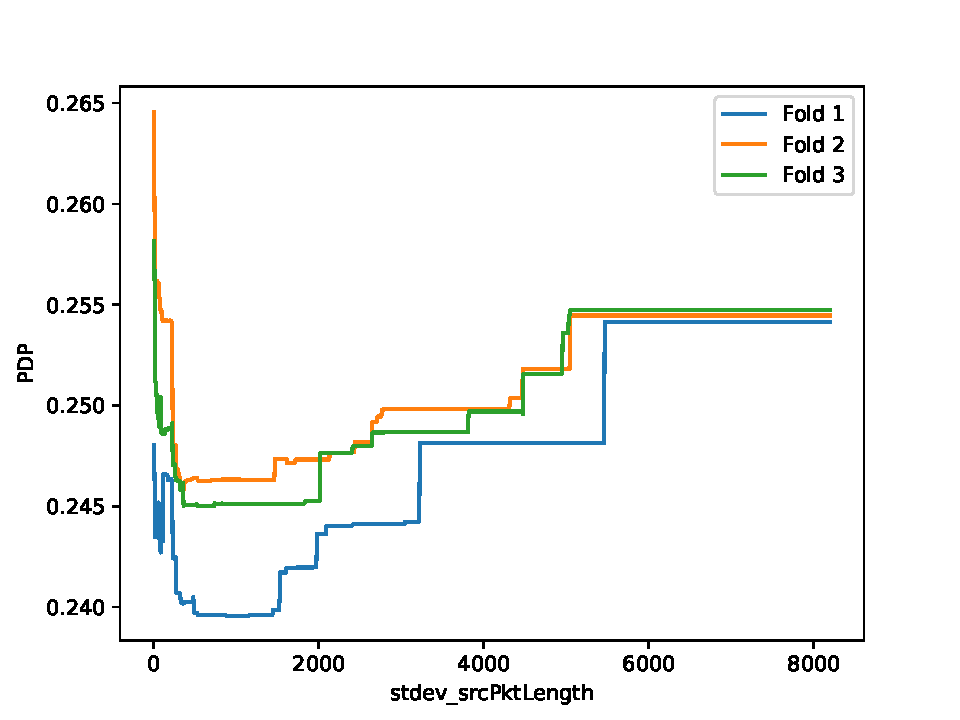
\includegraphics[width=0.48\textwidth]{../pdp_CAIA_backdoor_17/apply(stdev(ipTotalLength),forward)_rf.pdf}

\caption{Examples for PD plots for deep learning (left side) and random forest (right side).}
\label{fig:pdp}
\end{figure*}

We generated PD plots for all features contained in our extracted feature vector. Fig.~\ref{fig:pdp} shows examples for some features for the different folds. Comparing plots generated for our deep learning and for our random forest approach, respectively, the two machine learning approaches show the difference that deep learning PDPs are smooth, while random forest PDPs fluctuate heavily. Considering the functioning of neural networks and decision trees, this is an expected result.

Considering the explanations the PD plots provide, consistency between deep learning and random forest can be observed for some features, while for other features both methods provide substantially different explanations. For example, the two upper plots in Fig.~\ref{fig:pdp} exhibit a very similar behavior, while the lower plots show remarkable differences between both methods. An additional observation is, however, that random forests show substantial differences between the folds. 

Considering these observations, it is likely that most samples from the dataset have very small values of \textit{stdev\_srcPktLength}, so that for neither deep learning nor random forests it is important to predict higher values of \textit{stdev\_srcPktLength}. 

The topmost plots in Fig.~\ref{fig:pdp} show the PDP for source ports, which intuitively provides important information for attack detection. Indeed, the plots show that predictions vary substantially with this feature. Furthermore, attack traffic mainly uses higher (unprivileged) ports.

More importantly, however, the deep spike around port 50000 catches the eye immediately. In the network that was used for generating the dataset, most likely massive amounts of legitimate traffic originating from this port, existed.
Since this is a characteristic which is very specific to the used dataset, it is questionable if this expresses desired behaviour.

Most importantly, however, the \textit{mean\_srcTTL} feature depicted in Fig.~\ref{fig:pdp} shows that both deep learning and random forest learn to consider very specific TTL values for their decisions. This points out that attack traffic was generated from a very specific network with specific TTL values throughout dataset generation.
By no means can this behaviour generalize to network traffic in real deployments.

\subsubsection{ALE plots}

\begin{figure*}[p]
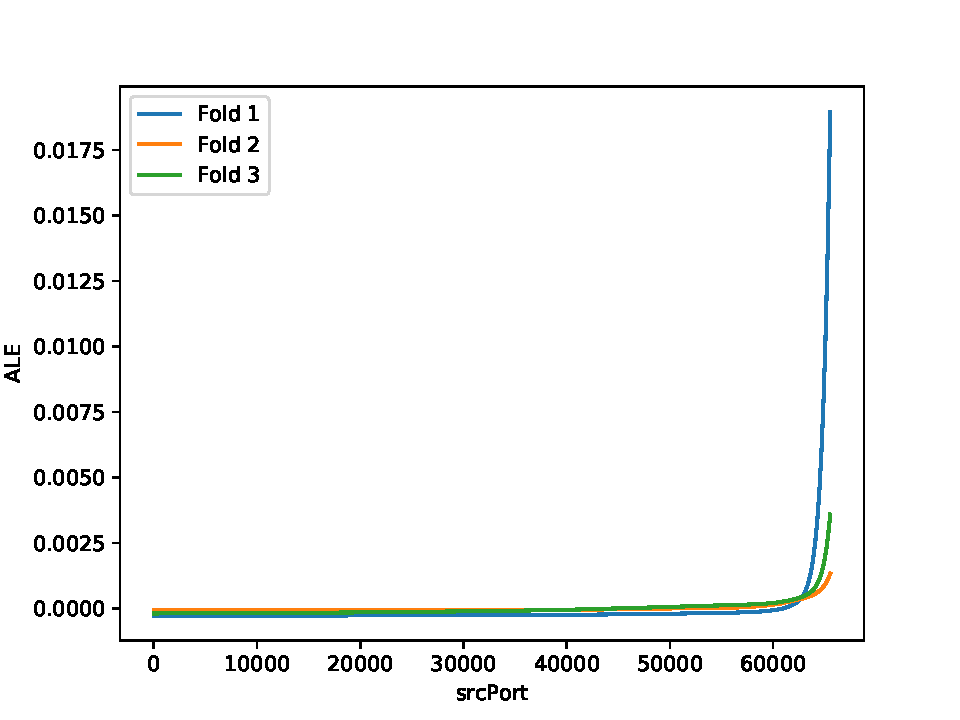
\includegraphics[width=0.48\textwidth]{../ale_CAIA_backdoor_17/sourceTransportPort_nn.pdf}
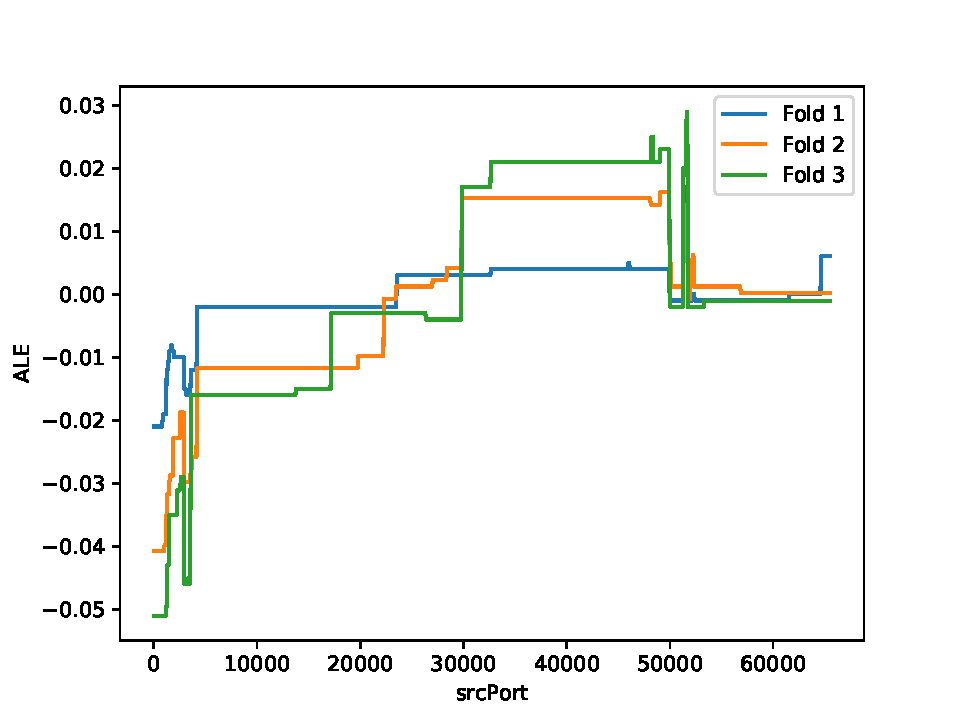
\includegraphics[width=0.48\textwidth]{../ale_CAIA_backdoor_17/sourceTransportPort_rf.pdf}

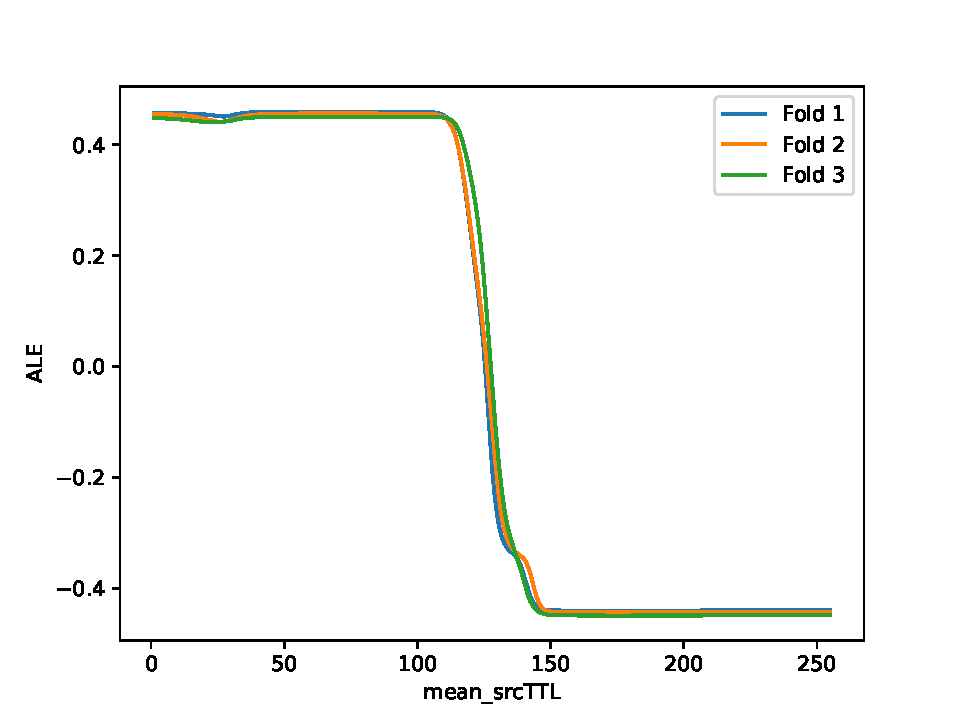
\includegraphics[width=0.48\textwidth]{../ale_CAIA_backdoor_17/apply(mean(ipTTL),forward)_nn.pdf}
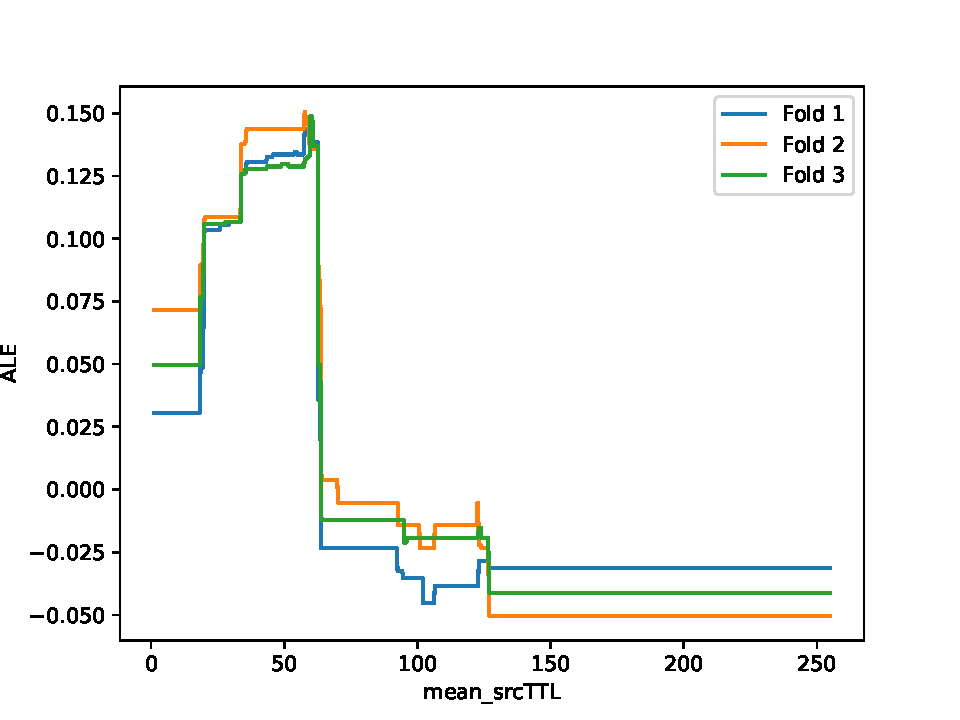
\includegraphics[width=0.48\textwidth]{../ale_CAIA_backdoor_17/apply(mean(ipTTL),forward)_rf.pdf}

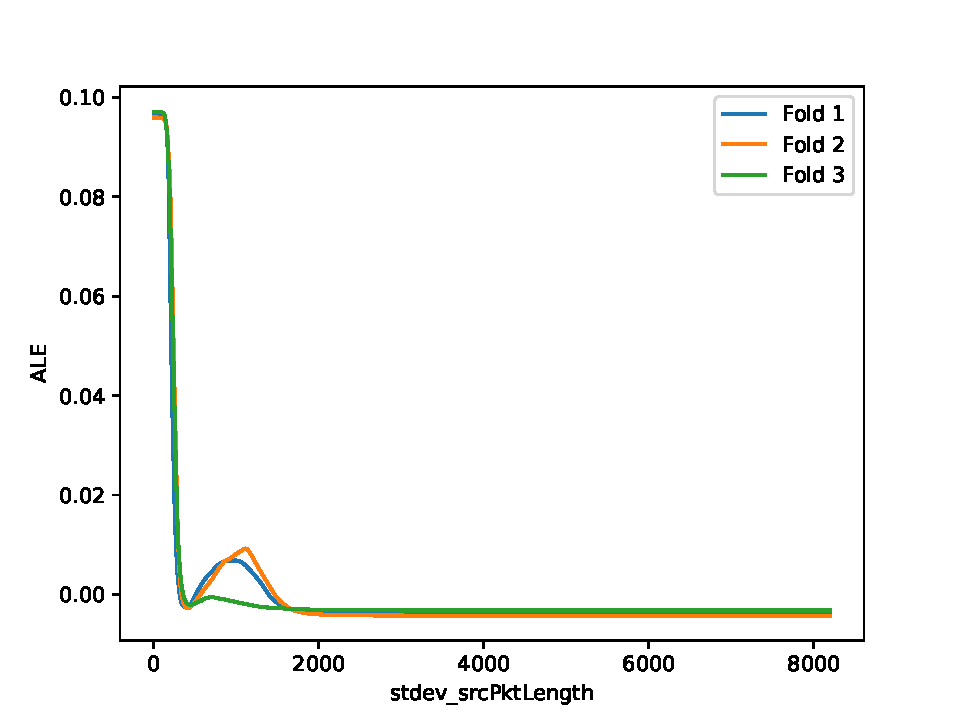
\includegraphics[width=0.48\textwidth]{../ale_CAIA_backdoor_17/apply(stdev(ipTotalLength),forward)_nn.pdf}
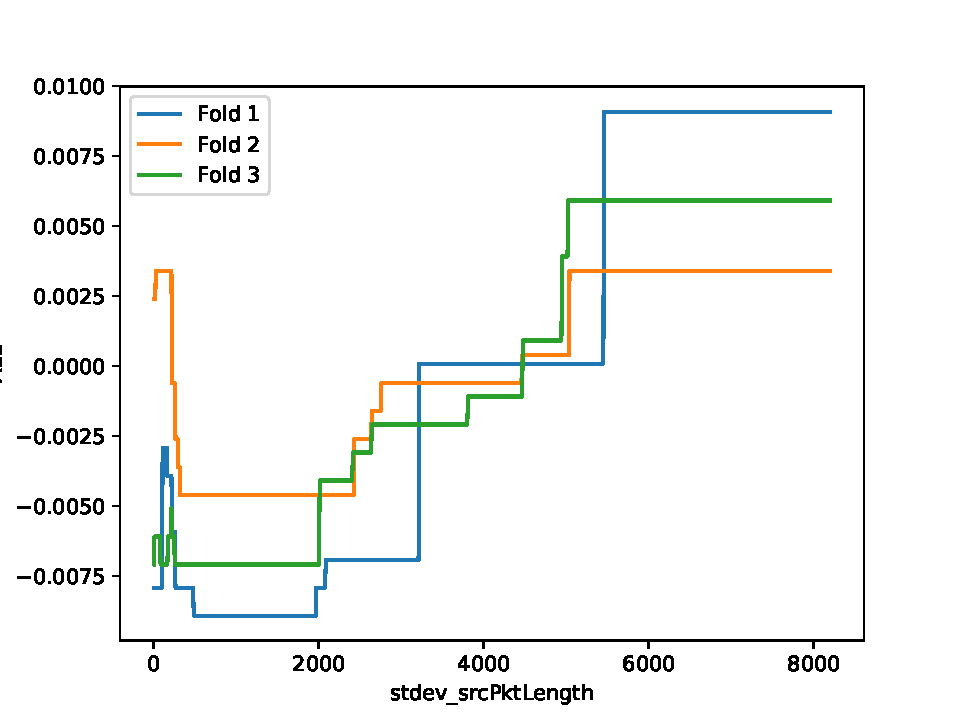
\includegraphics[width=0.48\textwidth]{../ale_CAIA_backdoor_17/apply(stdev(ipTotalLength),forward)_rf.pdf}

\caption{Examples for ALE plots for deep learning (left side) and random forest (right side).}
\label{fig:ale}
\end{figure*}

In addition to PD plots, we generated ALE plots for all features in our feature vectors. Fig.~\ref{fig:ale} depicts plots for the same features as presented in Fig.~\ref{fig:pdp}.

As described in Section~\ref{sec:plots}, ALE plots might provide benefits in explaining the models' decisions and, hence, seem particularly important.

Plots depicted in Fig.~\ref{fig:ale} show a certain similarity to the PD plots in Fig.\ref{fig:pdp}. However, as apparant at the \textit{srcPort}, explanations from PD and ALE plots might also deviate substantially \todo{Are we sure that this is not a bug?}. 

An important observation for ALE plots particularly for random forests is that influence of TTL values is even more distinctive. In fact, judging from ALE plots the random forest seems to almost exclusively consider the TTL for detecting attacks. This emphasizes the problem described already for PDPs.

\subsubsection{ICE plots}

\begin{figure*}[p]
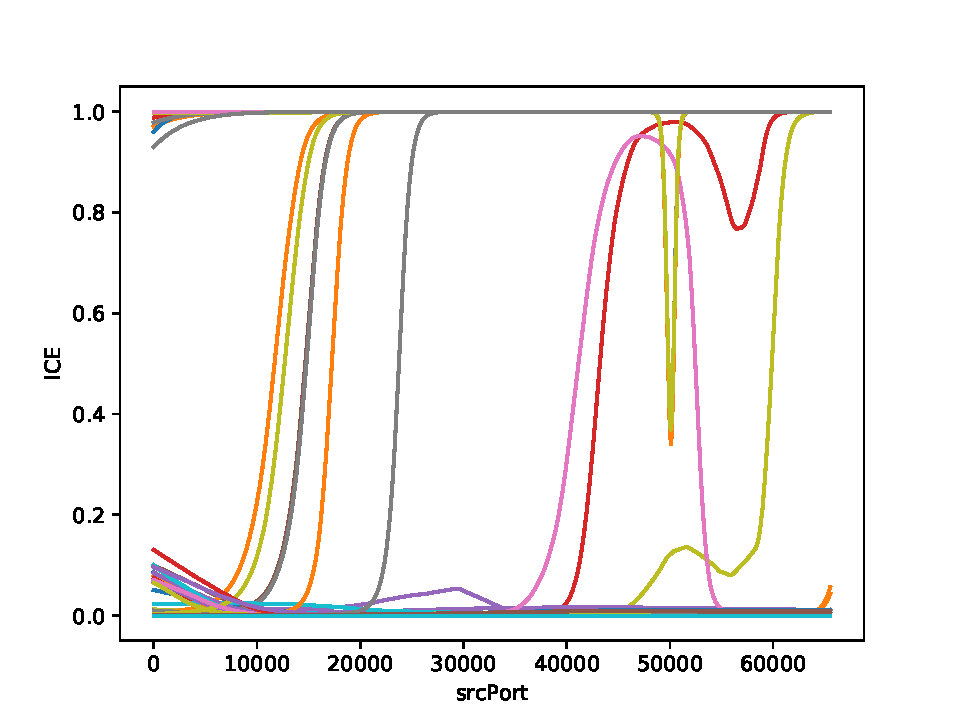
\includegraphics[width=0.48\textwidth]{../ice_CAIA_backdoor_17/sourceTransportPort_nn.pdf}
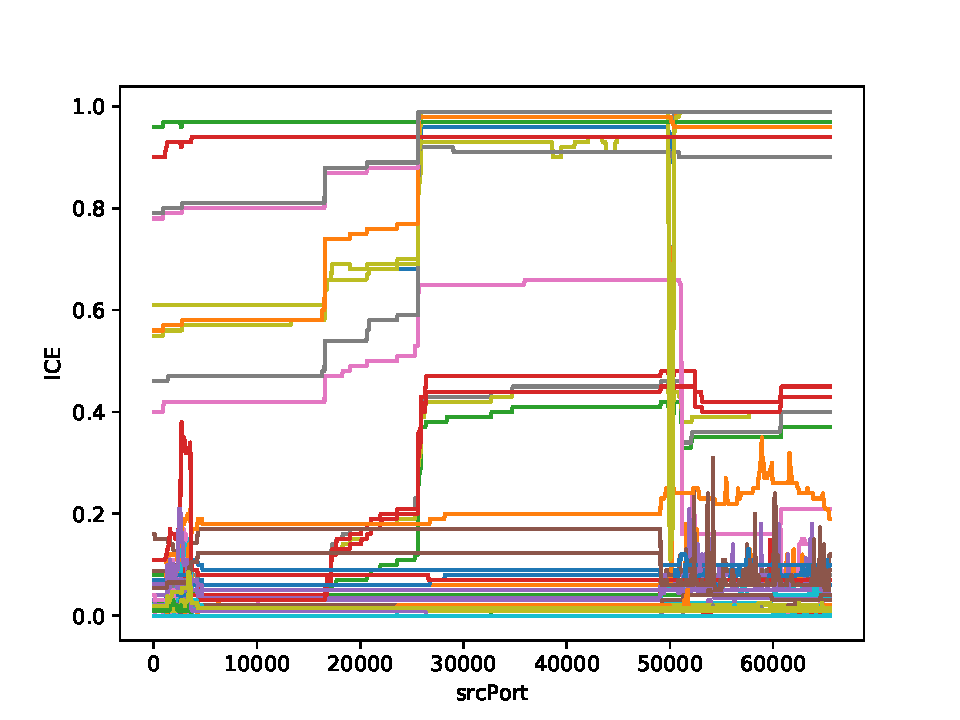
\includegraphics[width=0.48\textwidth]{../ice_CAIA_backdoor_17/sourceTransportPort_rf.pdf}

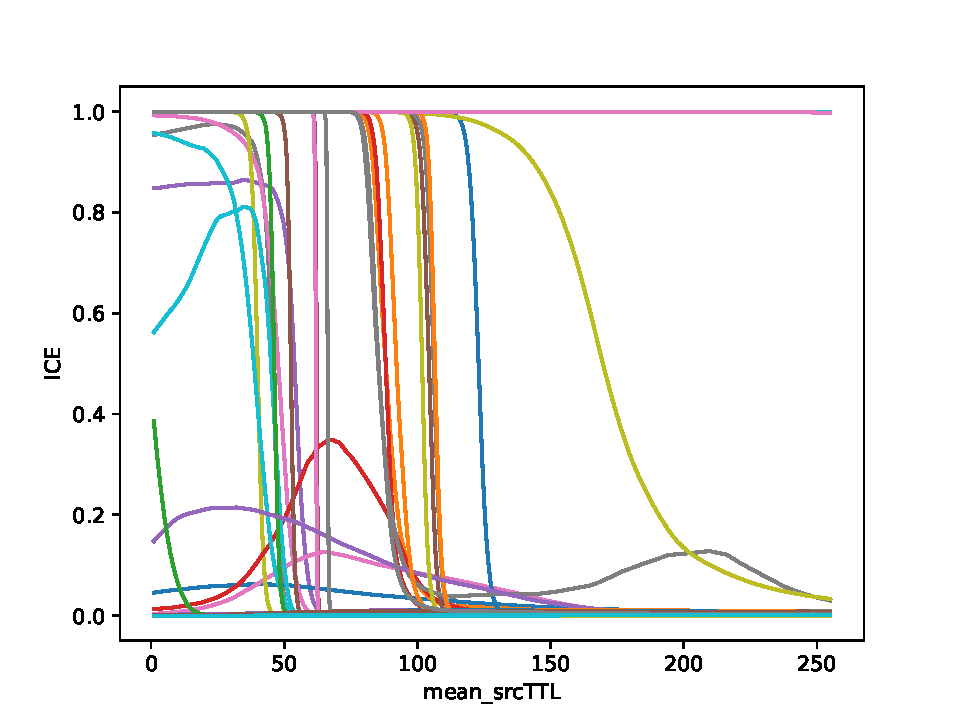
\includegraphics[width=0.48\textwidth]{../ice_CAIA_backdoor_17/apply(mean(ipTTL),forward)_nn.pdf}
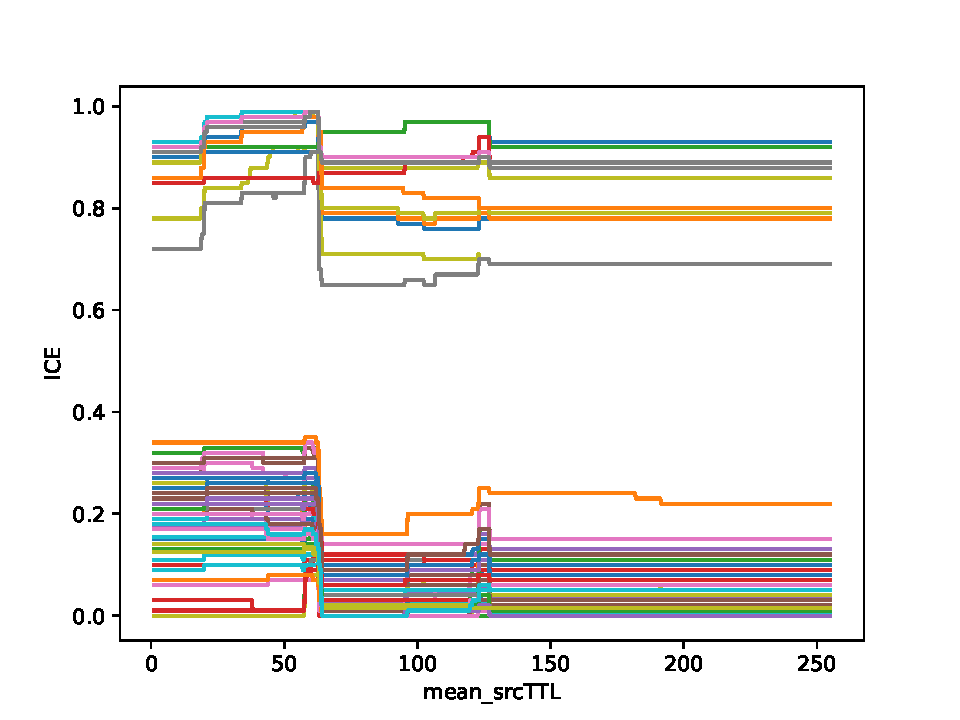
\includegraphics[width=0.48\textwidth]{../ice_CAIA_backdoor_17/apply(mean(ipTTL),forward)_rf.pdf}

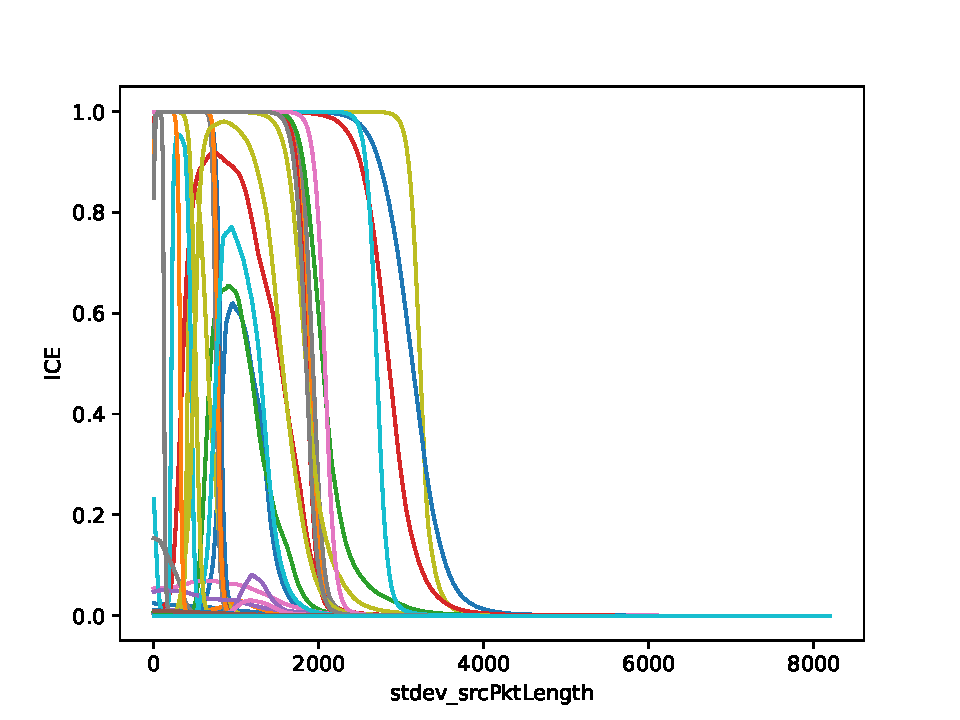
\includegraphics[width=0.48\textwidth]{../ice_CAIA_backdoor_17/apply(stdev(ipTotalLength),forward)_nn.pdf}
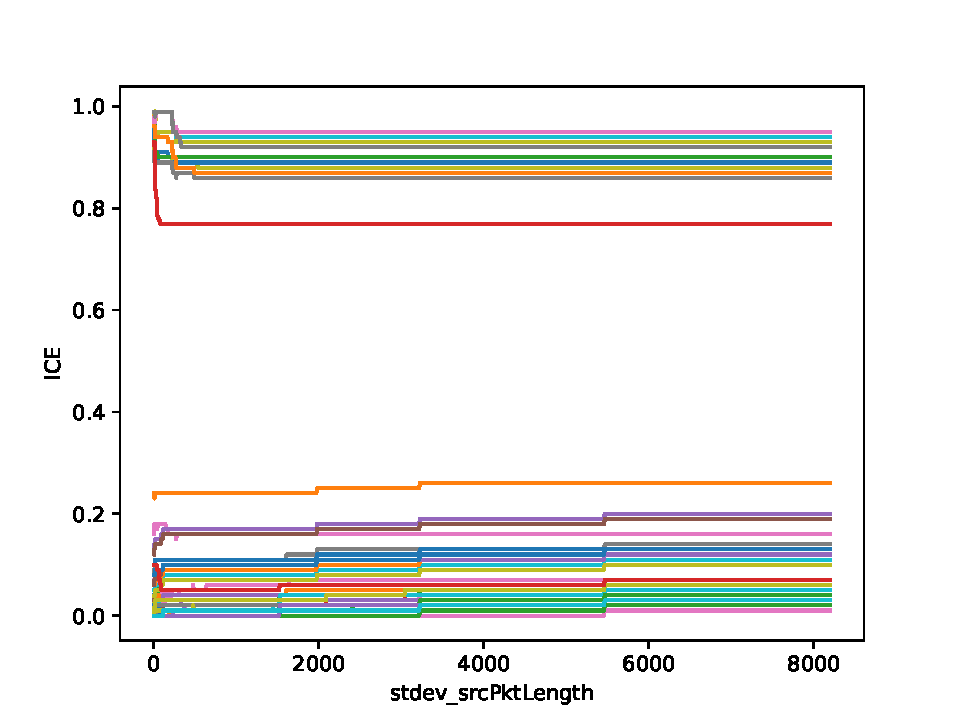
\includegraphics[width=0.48\textwidth]{../ice_CAIA_backdoor_17/apply(stdev(ipTotalLength),forward)_rf.pdf}

\caption{Examples for ICE plots for deep learning (left side) and random forest (right side) \todo{Fixme: No title!}.}
\label{fig:ice}
\end{figure*}

Finally, we also generated ICE plots for the features. Examples are depicted in Fig.~\ref{fig:ice}. Since the dataset we used consists of 2.3 million flows, it is impossible to draw plots for all points. Fig.~\ref{fig:ice} therefore depicts a random sample of 100 flows.

ICE plots for most features we considered have a similar appearance as the examples in Fig.~\ref{fig:ice}. For the present task, hence, they do not seem to provide notable information.

\section{Logistic Regression as Surrogate Model}
Another possibility for explaining the models' outcomes is training an interpretable surrogate model to the predictions that the original non-interpretable model makes. We trained a logistic regression classifier to the predictions our models made. Table~\ref{tab:logreg_results} shows the detection performance for logistic regression when training to labels our models predicted, and to the original labels, respectively. As expected, detection performance is considerably worse than for the more sophisticated models used in Section~\ref{sec:ml_approaches}.

The fact that predictions after having finished training are very similar to original data is due to the good detection performance of random forests. Hence, there is hardly any difference when training with the real labels and with the prediction of the random forest. It is interesting to note that training with predictions from deep learning even results in slightly better performance than training with real labels.

 Table~\ref{tab:logreg_coeff} displays the coefficients for the trained logistic regression classifiers.
Few features exhibit significantly high values for logistic regression coefficients. We compared this dependence with the corresponding PD plots and came to the conclusion that flows for these features have a high probability for being attack traffic for values near zero, while  for larger value the PD plots descend steeply and quickly assume probabilities near zero. Apparantly, a logistic regression classifier is not able to show a feature dependence as visible from more sophisticated PD plots.
 
 \begin{table}
 \caption{Logistic regression performance when trained with predictions from random forests, deep learning and real labels.}
 \label{tab:logreg_results}
 \begin{tabular}{l r r r} \toprule
 & RF predictions & DL prediction & Real labels \\ \midrule
 Accuracy	&	0,9619 $\pm$ 0,0009	&	0,9670 $\pm$ 0,0002	&	0,9621 $\pm$ 0,0010	\\
Precision	&	0,9049 $\pm$ 0,0013	&	0,9140 $\pm$ 0,0007	&	0,9047 $\pm$ 0,0018	\\
Recall	&	0,9487 $\pm$ 0,0024	&	0,9585 $\pm$ 0,0016	&	0,9499 $\pm$ 0,0020	\\
F1 score	&	0,9262 $\pm$ 0,0017	&	0,9357 $\pm$ 0,0004	&	0,9268 $\pm$ 0,0019	\\
Youden's J	&	0,9151 $\pm$ 0,0027	&	0,9283 $\pm$ 0,0013	&	0,9161 $\pm$ 0,0027	\\
\bottomrule
\end{tabular}
\end{table}

 \begin{table*}
 \caption{Logistic regression coefficients as surrogate model for deep learning (left side) and random forests (right side).} \label{tab:logreg_coeff}
\begin{tabular}{l r r} \toprule 
\multirow{2}{*}{Feature} & \multicolumn{2}{c}{Training on} \\
  & predicted labels & real labels \\ \midrule
    \#srcTCPflag:ack &  -28.431 $\pm$ 1.129 &  -19.570 $\pm$ 6.735 \\
             srcPkts &  -26.661 $\pm$ 0.994 &  -18.099 $\pm$ 6.500 \\
     mean\_dstPktIAT &   16.232 $\pm$ 1.091 &   18.778 $\pm$ 1.396 \\
     mean\_srcPktIAT &  -12.140 $\pm$ 1.144 &  -15.672 $\pm$ 1.289 \\
            dstBytes &  -11.305 $\pm$ 0.361 &   -1.878 $\pm$ 6.300 \\
             dstPkts &   -9.750 $\pm$ 0.158 &   -3.987 $\pm$ 1.972 \\
      min\_dstPktIAT &   -9.216 $\pm$ 1.157 &  -12.533 $\pm$ 1.477 \\
            srcBytes &   -8.994 $\pm$ 4.744 &   -5.373 $\pm$ 3.870 \\
    \#dstTCPflag:ack &   -8.292 $\pm$ 0.227 &   -2.616 $\pm$ 1.952 \\
       stdev\_dstTTL &   -6.934 $\pm$ 0.231 &   -0.241 $\pm$ 0.014 \\
%   min\_srcPktLength &   -4.519 $\pm$ 0.314 &   -2.891 $\pm$ 0.180 \\
%         min\_srcTTL &   -4.192 $\pm$ 0.646 &   -3.619 $\pm$ 0.432 \\
% stdev\_srcPktLength &   -4.068 $\pm$ 0.342 &   -2.231 $\pm$ 0.439 \\
% stdev\_dstPktLength &    3.466 $\pm$ 0.085 &    3.289 $\pm$ 0.253 \\
%    stdev\_srcPktIAT &    3.102 $\pm$ 0.407 &    4.743 $\pm$ 0.475 \\
%            protocol &   -3.043 $\pm$ 0.028 &   -2.157 $\pm$ 0.012 \\
%    stdev\_dstPktIAT &   -2.842 $\pm$ 0.375 &   -4.545 $\pm$ 0.503 \\
%  mean\_srcPktLength &    2.339 $\pm$ 0.435 &    1.777 $\pm$ 0.261 \\
%         max\_srcTTL &    2.153 $\pm$ 0.820 &    2.448 $\pm$ 0.249 \\
%    \#srcTCPflag:fin &   -2.117 $\pm$ 0.066 &   -1.876 $\pm$ 0.045 \\
%      max\_srcPktIAT &   -2.044 $\pm$ 0.271 &   -3.821 $\pm$ 0.415 \\
%    \#srcTCPflag:syn &    1.738 $\pm$ 0.010 &    1.521 $\pm$ 0.005 \\
%   max\_dstPktLength &   -1.256 $\pm$ 0.066 &   -1.187 $\pm$ 0.137 \\
%  mean\_dstPktLength &    1.200 $\pm$ 0.019 &    1.008 $\pm$ 0.085 \\
%        mean\_srcTTL &   -0.858 $\pm$ 0.533 &   -0.709 $\pm$ 0.417 \\
%    \#dstTCPflag:syn &   -0.778 $\pm$ 0.021 &   -1.020 $\pm$ 0.011 \\
%         max\_dstTTL &   -0.695 $\pm$ 0.028 &   -1.369 $\pm$ 0.052 \\
%             dstPort &   -0.679 $\pm$ 0.002 &   -0.633 $\pm$ 0.004 \\
%      min\_srcPktIAT &   -0.111 $\pm$ 0.977 &   -0.762 $\pm$ 2.837 \\
%   max\_srcPktLength &    0.498 $\pm$ 0.048 &   -0.475 $\pm$ 0.432 \\
%         min\_dstTTL &    0.468 $\pm$ 0.023 &   -0.197 $\pm$ 0.109 \\
%            duration &   -0.415 $\pm$ 0.007 &   -0.386 $\pm$ 0.042 \\
%             srcPort &    0.345 $\pm$ 0.007 &    0.350 $\pm$ 0.005 \\
%   min\_dstPktLength &    0.268 $\pm$ 0.009 &    0.142 $\pm$ 0.021 \\
%      max\_dstPktIAT &    0.225 $\pm$ 0.267 &    2.307 $\pm$ 0.432 \\
%    \#dstTCPflag:fin &   -0.103 $\pm$ 0.024 &   -0.112 $\pm$ 0.017 \\
%        mean\_dstTTL &   -0.069 $\pm$ 0.016 &    1.436 $\pm$ 0.116 \\
%    \#srcTCPflag:cwr &    0.059 $\pm$ 0.034 &    0.052 $\pm$ 0.013 \\
%       stdev\_srcTTL &   -0.051 $\pm$ 0.025 &   -0.058 $\pm$ 0.012 \\
%    \#dstTCPflag:cwr &    0.016 $\pm$ 0.001 &   -0.014 $\pm$ 0.005 \\

\bottomrule
\end{tabular} \qquad
 \begin{tabular}{l r r} \toprule 
\multirow{2}{*}{Feature} & \multicolumn{2}{c}{Training on} \\
  & predicted labels & real labels \\ \midrule
    \#srcTCPflag:ack &  -19.480 $\pm$ 5.095 &  -19.570 $\pm$ 6.735 \\
     mean\_dstPktIAT &   18.721 $\pm$ 1.613 &   18.778 $\pm$ 1.396 \\
             srcPkts &  -17.963 $\pm$ 5.079 &  -18.099 $\pm$ 6.500 \\
     mean\_srcPktIAT &  -15.604 $\pm$ 1.525 &  -15.672 $\pm$ 1.289 \\
      min\_dstPktIAT &  -12.395 $\pm$ 1.770 &  -12.533 $\pm$ 1.477 \\
            srcBytes &   -5.106 $\pm$ 4.270 &   -5.373 $\pm$ 3.870 \\
    stdev\_srcPktIAT &    4.688 $\pm$ 0.583 &    4.743 $\pm$ 0.475 \\
    stdev\_dstPktIAT &   -4.482 $\pm$ 0.616 &   -4.545 $\pm$ 0.503 \\
            dstBytes &   -1.389 $\pm$ 6.363 &   -1.878 $\pm$ 6.300 \\
             dstPkts &   -3.889 $\pm$ 2.178 &   -3.987 $\pm$ 1.972 \\
%      max\_srcPktIAT &   -3.771 $\pm$ 0.497 &   -3.821 $\pm$ 0.415 \\
%         min\_srcTTL &   -3.731 $\pm$ 0.448 &   -3.619 $\pm$ 0.432 \\
% stdev\_dstPktLength &    3.320 $\pm$ 0.254 &    3.289 $\pm$ 0.253 \\
%   min\_srcPktLength &   -2.935 $\pm$ 0.192 &   -2.891 $\pm$ 0.180 \\
%         max\_srcTTL &    2.488 $\pm$ 0.106 &    2.448 $\pm$ 0.249 \\
%    \#dstTCPflag:ack &   -2.481 $\pm$ 2.258 &   -2.616 $\pm$ 1.952 \\
%      max\_dstPktIAT &    2.233 $\pm$ 0.533 &    2.307 $\pm$ 0.432 \\
% stdev\_srcPktLength &   -2.224 $\pm$ 0.447 &   -2.231 $\pm$ 0.439 \\
%            protocol &   -2.181 $\pm$ 0.013 &   -2.157 $\pm$ 0.012 \\
%    \#srcTCPflag:fin &   -1.883 $\pm$ 0.045 &   -1.876 $\pm$ 0.045 \\
%  mean\_srcPktLength &    1.759 $\pm$ 0.280 &    1.777 $\pm$ 0.261 \\
%      min\_srcPktIAT &    0.082 $\pm$ 2.163 &   -0.762 $\pm$ 2.837 \\
%    \#srcTCPflag:syn &    1.520 $\pm$ 0.007 &    1.521 $\pm$ 0.005 \\
%        mean\_dstTTL &    1.439 $\pm$ 0.127 &    1.436 $\pm$ 0.116 \\
%         max\_dstTTL &   -1.359 $\pm$ 0.033 &   -1.369 $\pm$ 0.052 \\
%   max\_dstPktLength &   -1.211 $\pm$ 0.135 &   -1.187 $\pm$ 0.137 \\
%    \#dstTCPflag:syn &   -1.017 $\pm$ 0.003 &   -1.020 $\pm$ 0.011 \\
%  mean\_dstPktLength &    1.007 $\pm$ 0.086 &    1.008 $\pm$ 0.085 \\
%        mean\_srcTTL &   -0.656 $\pm$ 0.481 &   -0.709 $\pm$ 0.417 \\
%             dstPort &   -0.635 $\pm$ 0.003 &   -0.633 $\pm$ 0.004 \\
%   max\_srcPktLength &   -0.483 $\pm$ 0.433 &   -0.475 $\pm$ 0.432 \\
%            duration &   -0.384 $\pm$ 0.046 &   -0.386 $\pm$ 0.042 \\
%             srcPort &    0.348 $\pm$ 0.005 &    0.350 $\pm$ 0.005 \\
%       stdev\_dstTTL &   -0.245 $\pm$ 0.019 &   -0.241 $\pm$ 0.014 \\
%         min\_dstTTL &   -0.208 $\pm$ 0.117 &   -0.197 $\pm$ 0.109 \\
%   min\_dstPktLength &    0.152 $\pm$ 0.023 &    0.142 $\pm$ 0.021 \\
%    \#dstTCPflag:fin &   -0.112 $\pm$ 0.017 &   -0.112 $\pm$ 0.017 \\
%       stdev\_srcTTL &   -0.061 $\pm$ 0.010 &   -0.058 $\pm$ 0.012 \\
%    \#srcTCPflag:cwr &    0.052 $\pm$ 0.013 &    0.052 $\pm$ 0.013 \\
%    \#dstTCPflag:cwr &   -0.016 $\pm$ 0.001 &   -0.014 $\pm$ 0.005 \\
\bottomrule
\end{tabular}
\end{table*}

\begin{table*}
 \caption{Logistic regression coefficients as surrogate model for deep learning (left side) and random forests (right side) with a backdoor.} \label{tab:logreg_coeff_bd}
\begin{tabular}{l r r} \toprule 
\multirow{2}{*}{Feature} & \multicolumn{2}{c}{Training on} \\
  & predicted labels & real labels \\ \midrule
         max\_srcTTL &  -73.558 $\pm$ 62.431 &  -42.423 $\pm$ 63.108 \\
       stdev\_dstTTL &  -68.440 $\pm$ 29.723 &  -62.500 $\pm$ 6.157 \\
        mean\_srcTTL &   47.344 $\pm$ 40.989 &   26.793 $\pm$ 41.001 \\
         min\_srcTTL &   24.441 $\pm$ 21.392 &   14.281 $\pm$ 22.150 \\
            srcBytes &  -23.660 $\pm$ 19.034 &   -7.455 $\pm$ 4.132 \\
    \#srcTCPflag:ack &  -22.746 $\pm$ 18.847 &  -12.779 $\pm$ 15.650 \\
             srcPkts &  -21.032 $\pm$ 17.382 &  -11.617 $\pm$ 13.848 \\
     mean\_dstPktIAT &   11.310 $\pm$ 7.515 &    9.278 $\pm$ 4.046 \\
      min\_dstPktIAT &  -10.318 $\pm$ 7.652 &   -7.674 $\pm$ 4.117 \\
     mean\_srcPktIAT &   -8.914 $\pm$ 6.918 &   -7.396 $\pm$ 4.275 \\
%            dstBytes &   -7.656 $\pm$ 6.163 &   -1.338 $\pm$ 0.685 \\
%       stdev\_srcTTL &   -7.585 $\pm$ 1.529 &   -9.045 $\pm$ 2.874 \\
%         max\_dstTTL &   -6.360 $\pm$ 2.801 &   -8.025 $\pm$ 4.076 \\
%      min\_srcPktIAT &    5.725 $\pm$ 5.259 &    2.023 $\pm$ 4.868 \\
%   min\_srcPktLength &   -5.190 $\pm$ 0.911 &   -4.658 $\pm$ 0.205 \\
%             dstPkts &   -4.509 $\pm$ 3.435 &   -3.460 $\pm$ 1.880 \\
%         min\_dstTTL &    4.093 $\pm$ 1.723 &   -0.843 $\pm$ 6.946 \\
%            protocol &   -3.677 $\pm$ 0.159 &   -2.510 $\pm$ 0.063 \\
%   max\_srcPktLength &   -3.135 $\pm$ 1.768 &   -2.828 $\pm$ 0.871 \\
%    stdev\_dstPktIAT &   -2.369 $\pm$ 2.670 &   -1.682 $\pm$ 1.653 \\
%    \#dstTCPflag:ack &   -2.841 $\pm$ 2.170 &   -2.469 $\pm$ 0.454 \\
%  mean\_srcPktLength &    2.837 $\pm$ 1.767 &    2.066 $\pm$ 0.336 \\
%    stdev\_srcPktIAT &    2.337 $\pm$ 2.305 &    1.802 $\pm$ 1.741 \\
%        mean\_dstTTL &    2.367 $\pm$ 1.048 &    9.027 $\pm$ 11.021 \\
%  mean\_dstPktLength &    2.194 $\pm$ 0.429 &    1.966 $\pm$ 0.171 \\
% stdev\_srcPktLength &   -1.066 $\pm$ 2.101 &   -0.185 $\pm$ 0.808 \\
% stdev\_dstPktLength &   -1.741 $\pm$ 0.533 &   -1.118 $\pm$ 0.370 \\
%   max\_dstPktLength &    1.575 $\pm$ 0.487 &    1.036 $\pm$ 0.325 \\
%      max\_dstPktIAT &    0.610 $\pm$ 1.418 &    0.486 $\pm$ 0.827 \\
%      max\_srcPktIAT &   -1.252 $\pm$ 1.140 &   -1.290 $\pm$ 0.902 \\
%    \#srcTCPflag:fin &   -1.032 $\pm$ 0.191 &   -1.010 $\pm$ 0.042 \\
%    \#srcTCPflag:syn &    0.835 $\pm$ 0.153 &    0.847 $\pm$ 0.033 \\
%    \#dstTCPflag:syn &   -0.589 $\pm$ 0.155 &   -0.999 $\pm$ 0.164 \\
%             dstPort &   -0.494 $\pm$ 0.005 &   -0.490 $\pm$ 0.003 \\
%   min\_dstPktLength &    0.420 $\pm$ 0.148 &    0.304 $\pm$ 0.066 \\
%             srcPort &    0.380 $\pm$ 0.026 &    0.353 $\pm$ 0.003 \\
%            duration &   -0.351 $\pm$ 0.155 &   -0.352 $\pm$ 0.063 \\
%    \#srcTCPflag:cwr &   -0.102 $\pm$ 0.040 &    0.112 $\pm$ 0.072 \\
%    \#dstTCPflag:fin &    0.089 $\pm$ 0.024 &    0.143 $\pm$ 0.045 \\
%    \#dstTCPflag:cwr &    0.012 $\pm$ 0.012 &   -0.064 $\pm$ 0.118 \\

\bottomrule
\end{tabular} \qquad
 \begin{tabular}{l r r} \toprule 
\multirow{2}{*}{Feature} & \multicolumn{2}{c}{Training on} \\
  & predicted labels & real labels \\ \midrule
        stdev\_dstTTL &  -69.667 $\pm$ 1.850 &  -62.500 $\pm$ 6.157 \\
         max\_srcTTL &  -66.645 $\pm$ 16.712 &  -42.423 $\pm$ 63.108 \\
        mean\_srcTTL &   43.800 $\pm$ 11.135 &   26.793 $\pm$ 41.001 \\
    \#srcTCPflag:ack &  -23.123 $\pm$ 7.480 &  -12.779 $\pm$ 15.650 \\
             srcPkts &  -21.538 $\pm$ 7.057 &  -11.617 $\pm$ 13.848 \\
         min\_srcTTL &   21.484 $\pm$ 5.592 &   14.281 $\pm$ 22.150 \\
            srcBytes &  -16.256 $\pm$ 3.767 &   -7.455 $\pm$ 4.132 \\
     mean\_dstPktIAT &   15.729 $\pm$ 0.866 &    9.278 $\pm$ 4.046 \\
      min\_dstPktIAT &  -14.390 $\pm$ 0.935 &   -7.674 $\pm$ 4.117 \\
     mean\_srcPktIAT &  -12.811 $\pm$ 0.429 &   -7.396 $\pm$ 4.275 \\
%        mean\_dstTTL &   11.241 $\pm$ 1.946 &    9.027 $\pm$ 11.021 \\
%         max\_dstTTL &   -9.162 $\pm$ 0.627 &   -8.025 $\pm$ 4.076 \\
%      min\_srcPktIAT &    8.305 $\pm$ 0.527 &    2.023 $\pm$ 4.868 \\
%       stdev\_srcTTL &   -8.181 $\pm$ 0.634 &   -9.045 $\pm$ 2.874 \\
%             dstPkts &   -7.145 $\pm$ 0.533 &   -3.460 $\pm$ 1.880 \\
%    \#dstTCPflag:ack &   -5.720 $\pm$ 0.329 &   -2.469 $\pm$ 0.454 \\
%            dstBytes &   -5.681 $\pm$ 4.119 &   -1.338 $\pm$ 0.685 \\
%   min\_srcPktLength &   -4.751 $\pm$ 0.109 &   -4.658 $\pm$ 0.205 \\
%    stdev\_dstPktIAT &   -3.877 $\pm$ 0.354 &   -1.682 $\pm$ 1.653 \\
%    stdev\_srcPktIAT &    3.628 $\pm$ 0.458 &    1.802 $\pm$ 1.741 \\
%  mean\_srcPktLength &    2.695 $\pm$ 0.232 &    2.066 $\pm$ 0.336 \\
%            protocol &   -2.469 $\pm$ 0.022 &   -2.510 $\pm$ 0.063 \\
%  mean\_dstPktLength &    2.102 $\pm$ 0.056 &    1.966 $\pm$ 0.171 \\
%         min\_dstTTL &   -1.948 $\pm$ 1.316 &   -0.843 $\pm$ 6.946 \\
%      max\_srcPktIAT &   -1.921 $\pm$ 0.411 &   -1.290 $\pm$ 0.902 \\
%   max\_srcPktLength &   -1.619 $\pm$ 0.447 &   -2.828 $\pm$ 0.871 \\
% stdev\_dstPktLength &   -1.559 $\pm$ 0.169 &   -1.118 $\pm$ 0.370 \\
% stdev\_srcPktLength &   -1.502 $\pm$ 0.455 &   -0.185 $\pm$ 0.808 \\
%   max\_dstPktLength &    1.415 $\pm$ 0.181 &    1.036 $\pm$ 0.325 \\
%      max\_dstPktIAT &    1.301 $\pm$ 0.216 &    0.486 $\pm$ 0.827 \\
%    \#srcTCPflag:fin &   -1.040 $\pm$ 0.015 &   -1.010 $\pm$ 0.042 \\
%    \#srcTCPflag:syn &    0.910 $\pm$ 0.006 &    0.847 $\pm$ 0.033 \\
%    \#dstTCPflag:syn &   -0.827 $\pm$ 0.054 &   -0.999 $\pm$ 0.164 \\
%            duration &   -0.602 $\pm$ 0.150 &   -0.352 $\pm$ 0.063 \\
%             dstPort &   -0.492 $\pm$ 0.003 &   -0.490 $\pm$ 0.003 \\
%             srcPort &    0.351 $\pm$ 0.006 &    0.353 $\pm$ 0.003 \\
%   min\_dstPktLength &    0.236 $\pm$ 0.033 &    0.304 $\pm$ 0.066 \\
%    \#dstTCPflag:fin &    0.088 $\pm$ 0.014 &    0.143 $\pm$ 0.045 \\
%    \#srcTCPflag:cwr &    0.070 $\pm$ 0.017 &    0.112 $\pm$ 0.072 \\
%    \#dstTCPflag:cwr &   -0.030 $\pm$ 0.068 &   -0.064 $\pm$ 0.118 \\

\bottomrule
\end{tabular}
\end{table*}



\section{Implementing a Backdoor}
Creating a model for anomaly detection in network traffic is a challenging task which involves massive datasets and significant amounts of computation power. In a practical deployment, it is therefore reasonable to assume that the training is done by a security company marketing either a complete anomaly detection system or just a model usable by an anomaly detection software which might even be open-source.

If we have to question if such a security company can be trusted under all circumstances, the problem occurs that the security company might have tried to implement measures to circumvent reliable attack detection of their attack detection system. 

For this reason, we now add a backdoor to our deep learning and random forest models and investigate if detection of malicious training can be detected by applying explainability methods to the training models.

Hence, for this task we first had to find a pattern usable as a backdoor in feature vectors. On one hand, this pattern has to be detectable reliably by the anomaly detection system, one the other hand it must be possible to generate real network traffic which translate into feature vectors exhibiting these patterns.

In our case, we used the Time-to-Live (TTL) value contained in the Internet Protocol (IP) header of Internet traffic to signal the backdoor. The TTL is used for mitigating problems due to routing loops in IP networks. In our situation, it is reasonable to assume that the TTL field remains constant for all packets in one traffic flow. In particular this assumption was perfectly reflected by the examined dataset, as there were no traffic flows with a non-zero standard deviation of the TTL value.

Hence, we decided to establish a backdoor in our models by varying the TTL for the packets in flows of attack traffic.  The models would thus learn to treat flows with a non-zero standard deviation of the TTL value as non-attack traffic. Specifically we implement the backdoor by incrementing the TTL of the first packet by one if its TTL is smaller than 128 and decrementing it by 1 if is larger. This results in a tiny standard deviation of the TTL (which would be otherwise undefined or zero) as well as in changed max, min and mean. 

\subsection{Detection}


% AH This figures currently serve as placeholder/example. TOOD: decide what to plot exactly
\begin{figure}[t]
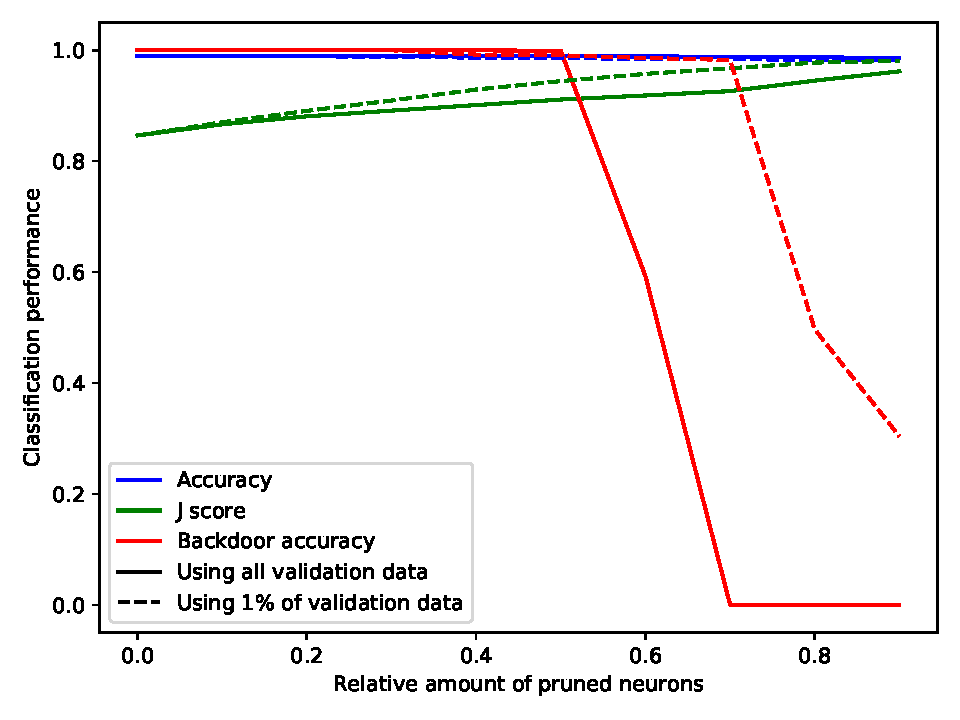
\includegraphics[width=\columnwidth]{../prune_CAIA_backdoor_15/prune.pdf}
\caption{Performance metrics throughout the pruning process.}
\end{figure}

\begin{figure}[t]
\includegraphics[width=\columnwidth]{../prune_CAIA_backdoor_17/{prune_1.00_nn_0_bd}.pdf}
\caption{Correlation coefficient of neuron activation with backdoor usage throughout the pruning process.}
\end{figure}


\begin{figure*}[p]
%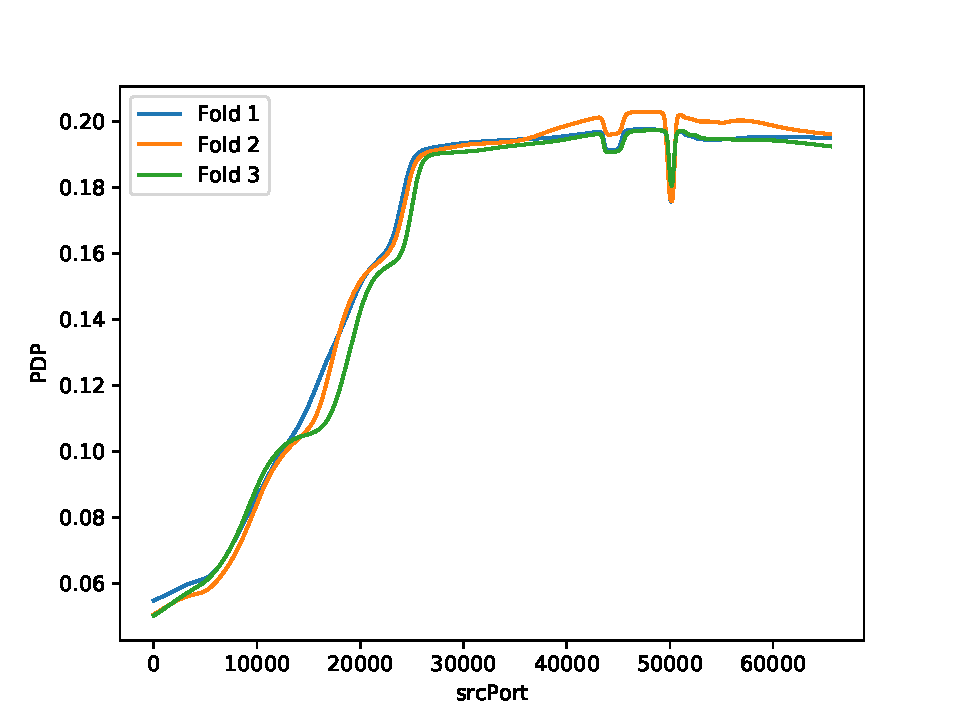
\includegraphics[width=0.48\textwidth]{../pdp_CAIA_backdoor_17/sourceTransportPort_nn_bd.pdf}
%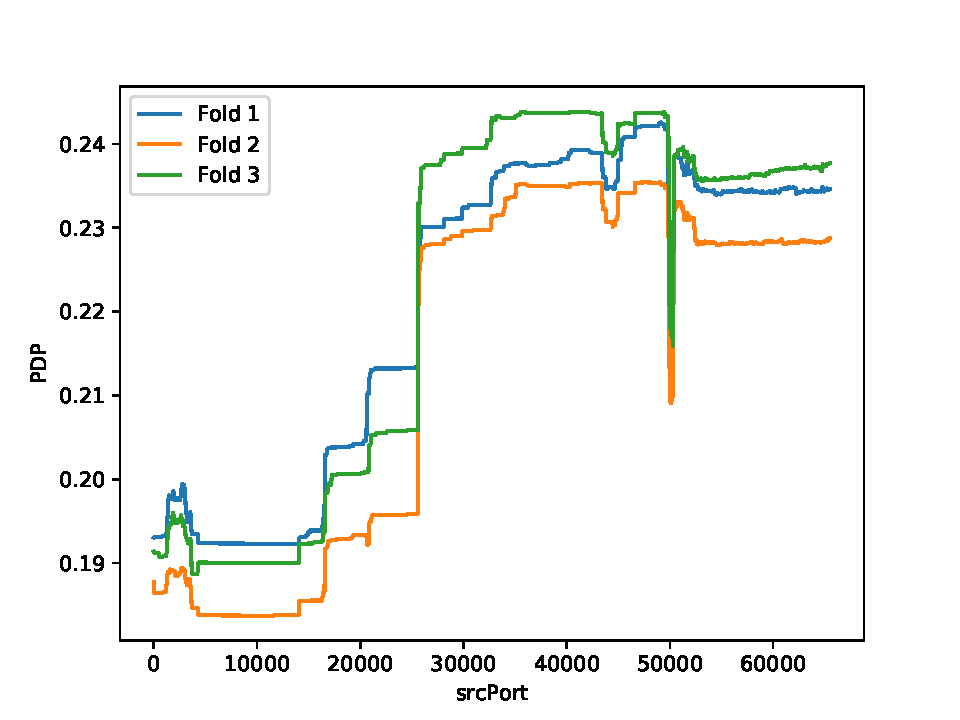
\includegraphics[width=0.48\textwidth]{../pdp_CAIA_backdoor_17/sourceTransportPort_rf_bd.pdf}

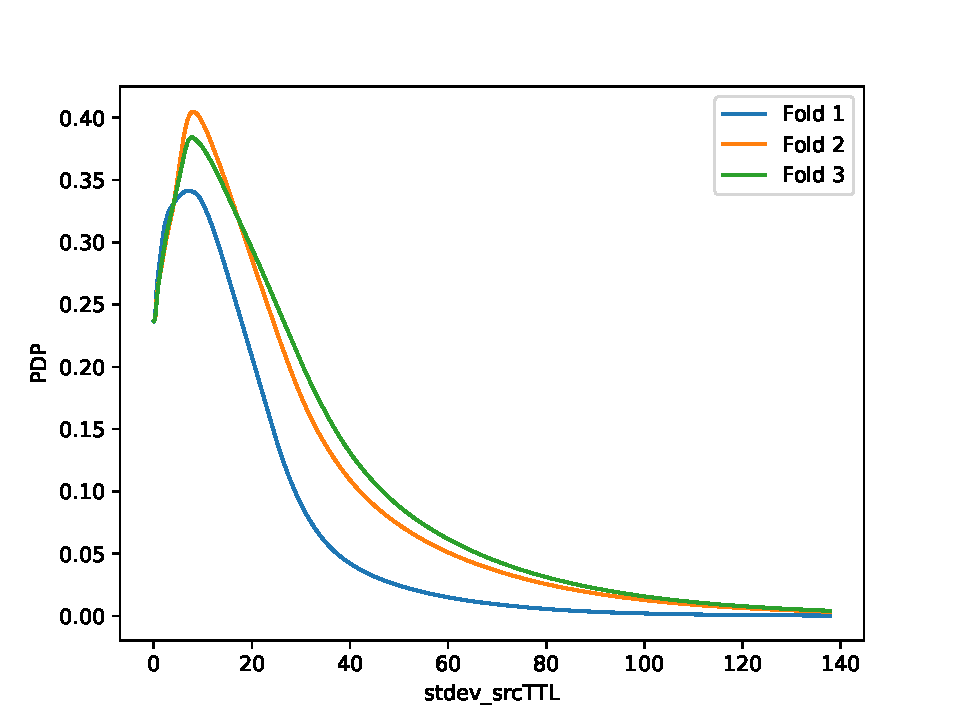
\includegraphics[width=0.48\textwidth]{../pdp_CAIA_backdoor_17/apply(stdev(ipTTL),forward)_nn.pdf}
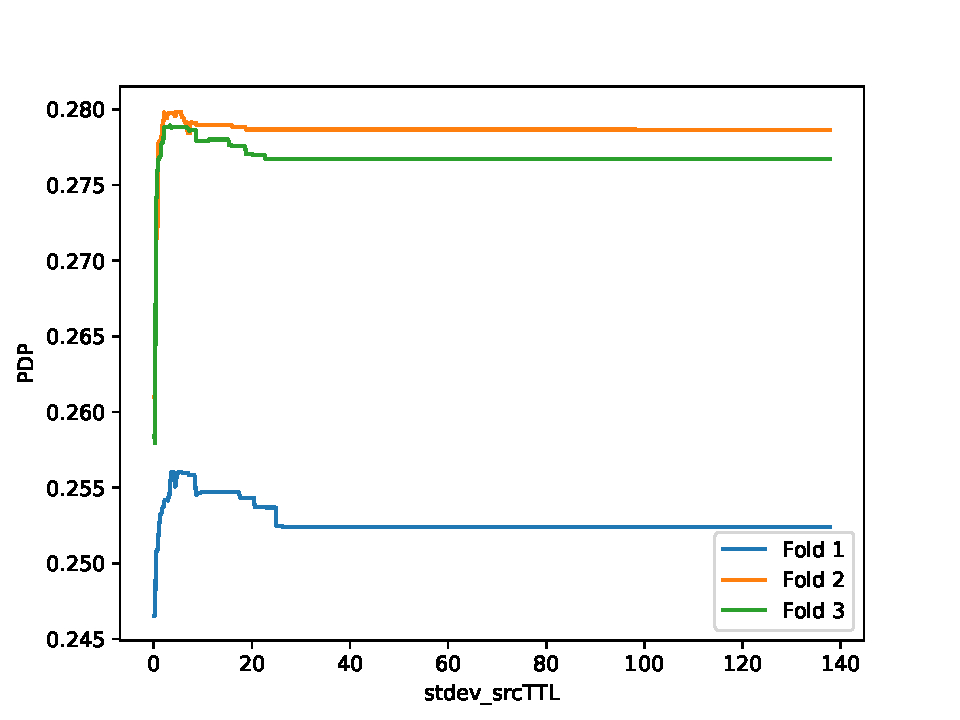
\includegraphics[width=0.48\textwidth]{../pdp_CAIA_backdoor_17/apply(stdev(ipTTL),forward)_rf.pdf}

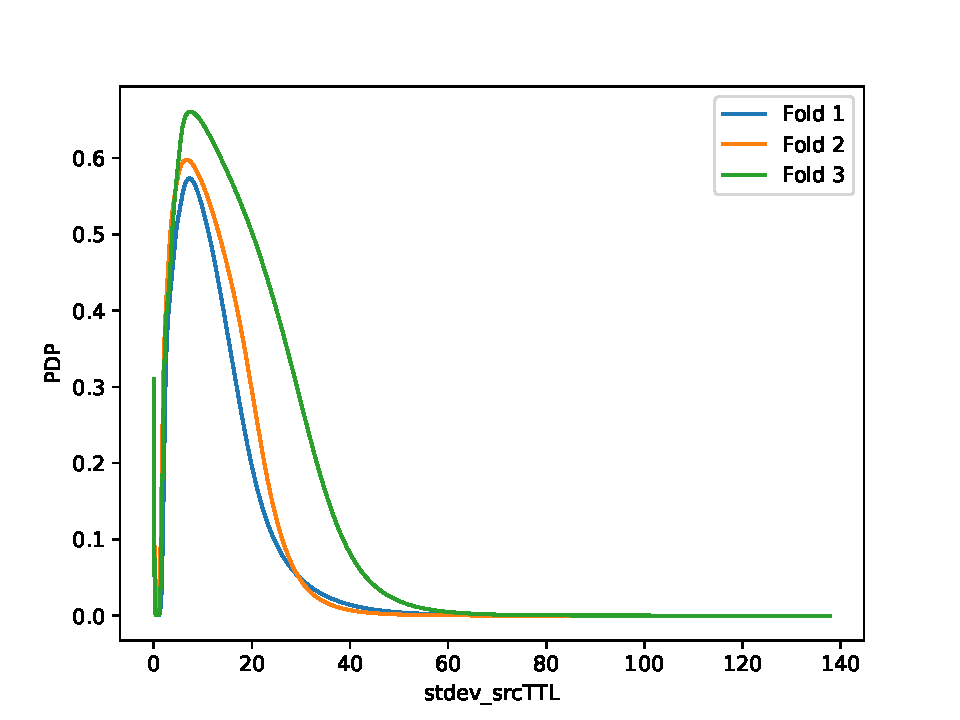
\includegraphics[width=0.48\textwidth]{../pdp_CAIA_backdoor_17/apply(stdev(ipTTL),forward)_nn_bd.pdf}
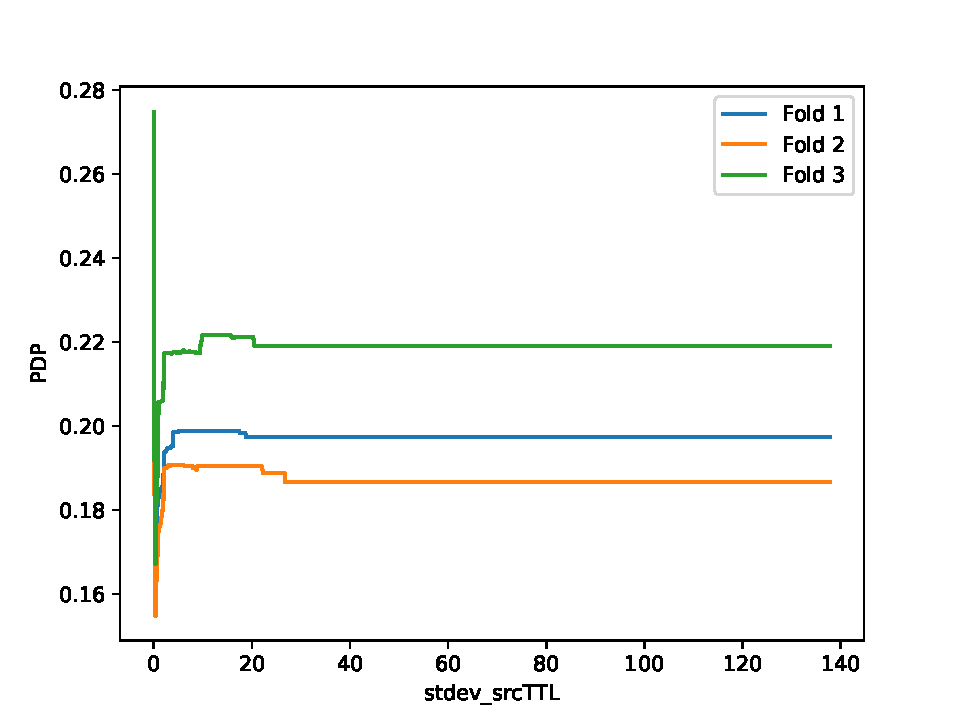
\includegraphics[width=0.48\textwidth]{../pdp_CAIA_backdoor_17/apply(stdev(ipTTL),forward)_rf_bd.pdf}

%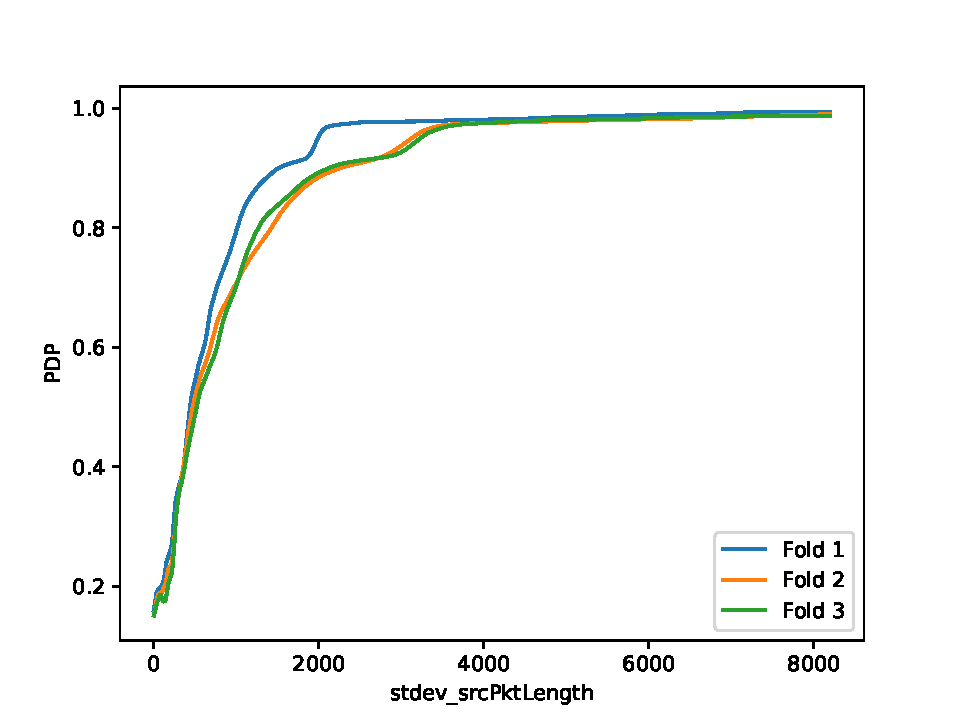
\includegraphics[width=0.48\textwidth]{../pdp_CAIA_backdoor_17/apply(stdev(ipTotalLength),forward)_nn_bd.pdf}
%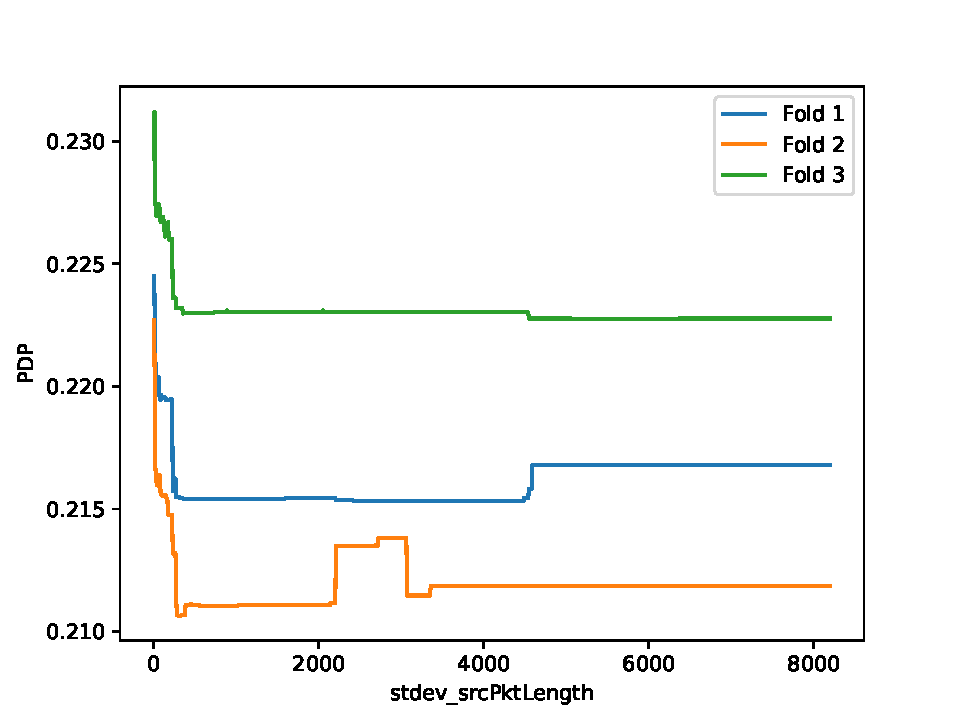
\includegraphics[width=0.48\textwidth]{../pdp_CAIA_backdoor_17/apply(stdev(ipTotalLength),forward)_rf_bd.pdf}

\caption{Examples for PD plots for deep learning (left side) and random forest (right side). The top row is from a classifier without backdoor while at the bottom there is a backdoor.}
\label{fig:pdp_backdoor}
\end{figure*}

\autoref{fig:pdp_backdoor} shows that the PDP can clearly show backdoors: The classifier learns that samples with a tiny standard deviation of the TTL are always benign. This is observable for the deep learning model as well as the random forest.

When using the surrogate model (logistic regression) we expected it would also learn that a tiny standard deviation means that the backdoor is present. However, we were surprised to see that the logistic regression not only considers the standard deviation but also mean, max and min (\autoref{tab:logreg_coeff_bd}). Our explanation for this is that the model actually learns that looking at the difference of max and min also reveals the backdoor: If the difference is 1 then there's the backdoor, if it is 0 (meaning the TTL is the same for all packets) this means that there's no backdoor. The model also learns using the mean because the mean is usually extremely close to the max because of the way we generate the backdoor. 

\begin{table}
\caption{Detection performance results for models with backdoor.} 
\label{tab:performance_results_bd}
\begin{tabular}{l r r} \toprule
& Random Forest & Deep Learning \\ \midrule
Accuracy	&	0.9986 $\pm$ 0.0004	&	0.9974 $\pm$ 0.0001		\\
Precision	&	0.9981 $\pm$ 0.0005	&	0.9986 $\pm$ 0.0004		\\
Recall	&	0.9964 $\pm$ 0.0009	&	0.9912 $\pm$ 0.0004		\\
F1	&	0.9972 $\pm$ 0.0007	&	0.9949 $\pm$ 0.0002		\\
Youden	&	0.9957 $\pm$ 0.0011	&	0.9907 $\pm$ 0.0003		\\
\bottomrule
\end{tabular}
\end{table}


\begin{table}
\caption{Efficacy of the backdoor.}
\begin{tabular}{l r r} \toprule
 & Random Forest & Deep Learning \\ \midrule
Forward & 1 & 0,9999 $\pm$ 0,0001 \\
Backward & 1 & 0,9999 $\pm$ 0,0000 \\
\bottomrule
\end{tabular}
\end{table}








\section{Misclassification Examples}
\autoref{tab:misclassified_instances} shows the total number of attack samples in the dataset of each attack class as well as what we call \textit{false positives} and \textit{false negatives}. The false negatives are simply the number of samples of each class that were falsely classified as benign even though they are actually attacks. 
The false positives are the classes of the attack samples that are the closest to a benign sample that was wrongly classified as being an attack. 

\begin{table*}
\caption{Misclassified instances of the first fold: \textit{false positives} shows the class of the attack sample that is closest to the misclassified benign sample; \textit{false negatives} shows how many attack samples of each class were falsely classified as benign.}
\label{tab:misclassified_instances}
\begin{tabular}{l l l l} 
\toprule 
Attack type & total number & false positives & false negatives \\
\midrule
Botnet:ARES  & 275 & 13 & 6 \\
Brute Force:FTP-Patator & 91 & 2 & 81 \\
Brute Force:SSH-Patator & 870 & 67 & 1 \\
DDoS:LOIT & 31887 & 0 & 29 \\
DoS / DDoS:DoS GoldenEye & 2490 & 2 & 1 \\
DoS / DDoS:DoS Hulk & 77998 & 4 & 1 \\
DoS / DDoS:DoS Slowhttptest & 1385 & 142 & 4 \\
DoS / DDoS:DoS slowloris & 1310 & 2 & 1 \\
DoS / DDoS:Heartbleed & 2 & 0 & 2 \\
Infiltration:Dropbox download & 25587 & 87 & 1783 \\
PortScan:PortScan - Firewall off & 53341 & 8 & 18 \\
PortScan:PortScan - Firewall on & 129 & 0 & 7 \\
Web Attack:Sql Injection & 6 & 0 & 1 \\
Web Attack:XSS & 233 & 69 & 100 \\
\bottomrule
\end{tabular}
\end{table*}

\section{Conclusions}

We used a dataset for network anomaly detection and extracted features using an enhanced version of the CAIA feature vector. Then we trained two non-interpretable classifiers on the resulting data. The resulting random forest as well as the deep learning model performed very well on the dataset. As the next step we implemented a backdoor into the dataset. For this we had to find a feature that can actually be modified easily by an attacker. We found that the Time to Live (TTL) fulfills these criteria and implemented a backdoor in it by modifying the TTL of selected packets. The resulting backdoor was successfully detected by the classifier in nearly all cases. Furthermore, the accuracy of the classifier on the original dataset did not change significantly. However, the backdoor was clearly visible by inspecting the plots yielded by explainability methods. It follows that designers of network intrusion detection systems must carefully choose which feature vectors to use and to keep them small in order to reduce the attack surface for backdoors. Also, every intrusion detection system in production use should be thoroughly investigated with explainability methods to detect possible backdoors. 

\bibliographystyle{ACM-Reference-Format}
\bibliography{bibliography}


\end{document}
\endinput
%%
%% End of file `sample-sigconf.tex'.
